\documentclass[11pt,a4paper]{report}
\setcounter{tocdepth}{2}
\usepackage[spanish]{babel}
\usepackage[utf8]{inputenc}
\usepackage{pdflscape}
\usepackage{hyperref}
\usepackage{geometry}
\usepackage[table,xcdraw]{xcolor}
\usepackage{float}
\usepackage{xcolor}
\usepackage{pgfplots}
\usepackage{listings}
\lstset{basicstyle=\ttfamily,
	showstringspaces=false,
	commentstyle=\color{red},
	keywordstyle=\color{blue}
}
\geometry{
	a4paper,
	total={170mm,257mm},
	left=20mm,
	top=20mm,
}
\usepackage{universityTitle}
\project{
	{\small Gestión de Proyecto Software,}\\
	{\small Departamento de Ingeniería e Informática de Sistemas,}\\
	{\small Universidad de Zaragoza}
}

\author{\textit{Equipo 1: GimnasIO
		\\Martínez Menéndez, Alberto %- 681061
		\\Navarro Castillo, Alejandro %- XXXXXX
 		\\Salueña Sediles, Asier %- 610344
 		\\Sánchez Salvador, Darío %- 680239
 	}}
\title{\textbf{Informe final del proyecto}}
\date{08 de enero, 2018}



\begin{document}
\maketitle
\titlepage
\begin{abstract}
	En este documento se detalla el proceso seguido durante el desarrollo de la app para móviles GimnasIO, la aplicación que te permite disponer de todas tus rutinas en tu Smartphone. Cada vez mas gente hace uso de los gimnasios y un alto porcentaje de estas personas desconoce los fundamentos de la práctica deportiva sin tener claro los objetivos de los ejercicios que puede proponer el monitor, o como distribuirlos en su sesión de entrenamiento, GimnasIO pretende suplir este déficit y servir de soporte a todas aquellas personas que quieren iniciarse en el mundo de la práctica deportiva en un gimnasio.
\end{abstract}
\newpage
\tableofcontents
\chapter{Introducción}
El proyecto que se ha llevado a cabo es una aplicación móvil desarrollada para OS Android cuyo objetivo es servir de soporte en la practica deportiva en gimnasios, esta aplicación denominada \textbf{GimnasIO} permite a los usuarios visualizar una colección de ejercicios y consultar distinta información de los mismos (principal musculo trabajado, otros músculos secundarios una descripción de su ejecución y una imagen del desarrollo del mismo), además permite a partir de estos ejercicios crear una rutina de ejercicios con un objetivo y un numero de series y repeticiones así como el descanso que requieren.
\newline
\\Este proyecto ha sido desarrollado por el equipo 1 de la asignatura Gestión de Proyecto Software de la Universidad de Zaragoza, este equipo esta formado por cuatro miembros siendo tres de ellos estudiantes de la rama de \textit{Ingeniería del Software } y el último de la rama de \textit{Tecnologías de la Información}, lo que aporta dos visiones al proyecto, una versión mas precisa del proceso de ingeniería en el desarrollo de un software y la visión del mundo IT.
\newline
\\El documento consta de dos secciones principales además de la sección de introducción y la de conclusiones, en las dos secciones principales se detallan toda la información referente al producto en primer caso y al proceso de desarrollo del proyecto en segundo caso.
\newline
\\En la sección que detalla la información referente al producto, se encuentra la información sobre el plan de producto y la planificación de lanzamientos, el análisis de riesgos llevado a cabo por el equipo en el desarrollo del producto, la pila de producto planteada hasta la finalización del primer sprint detallando a continuación el estado actual de la aplicación (funcionalidad implementada, GUI, aspectos de usabilidad, problemas conocidos...), por último se explica la arquitectura de la aplicación así como detalles sobre implementación y despliegue de la misma.
\newline
\\En la sección que contiene la información del proceso de desarrollo se detallan las estrategias de testing, y de automatización de despliegue, la definición de hecho con las mejoras realizadas a la definición inicial tras la revisión del profesorado, una breve explicación del sistema de control de versiones utilizado, información sobre los esfuerzos realizados así como un diagrama del trabajo completado/pendiente y un calculo de la velocidad del equipo, un análisis de resultados de la última retrospectiva y otros aspectos referentes a la gestión del proyecto que pudieran ser interesantes.
\chapter{Producto}
\section{Primer Sprint}
\subsection{Plan de producto y planificación de lanzamientos}
GimnasIO es una aplicación para Android que permite organizar las rutinas de gimnasio. La aplicación permite mantener una serie de rutinas guardadas, las cuales están compuestas de ejercicios seleccionados previamente durante su creación. Cada ejercicio viene acompañado de una explicación textual del mismo, así como de una imagen para que el usuario pueda observar cómo se realiza correctamente dicho ejercicio. La aplicación cuenta además con un reloj/contador para facilitar el control del tiempo de descanso o de la duración de determinados ejercicios.
\\Para la monetización de la aplicación se ha pensado la puesta en contacto con gimnasios y centros deportivos para que puedan crear sus rutinas privadas, permitiendo que sólo sus clientes tengan acceso mediante una clave a dichas rutinas más complejas y personalizadas. Los gimnasios y centros deportivos deberán abonar una suscripción para poder utilizar este servicio.
\newline Los requisitos a alto nivel de la aplicación son:
\begin{itemize}
	\item Se debe poder consultar la lista de ejercicios de la aplicación.
	\item Se debe poder crear una rutina de ejercicios, la cual consiste en un conjunto de ejercicios.
	\item Debe existir una forma de seguir una rutina en tiempo real (ejercicio actual, medición de tiempos de
	descanso, tiempo total, etc.)
	\item Se debe poder acceder a la aplicación sin conexión a Internet, pero limitando los servicios.
	\item La conexión a Internet será necesaria cuando se acceda por primera vez a la aplicación, haya alguna
	actualización de algún ejercicio o se acceda a una rutina privada de gimnasio.	
	\item Debe ser ejecutable en dispositivos Android.
\end{itemize}
Con respecto a los lanzamientos, se han determinado varias fechas de lanzamiento:
\begin{itemize}
	\item Una primera fecha de lanzamiento, el 24 de noviembre, que coincide con la finalización del primer sprint, cuya duración fue desde el 20 de octubre al 24 de noviembre de 2017. Para esta fecha de lanzamiento, el objetivo es presentar una aplicación con las funcionalidades básicas de modificación de rutinas (adición, edición, borrado), y la  vista y descarga de ejercicios de ejercicios desde un servidor remoto.
	\item Una segunda fecha de lanzamiento, el 30 de enero de 2018,  que coincide con la fecha de finalización del segundo sprint. En esta versión del producto, el objetivo es rehacer la GUI para que siga las guías de estilo y usabilidad de Android, implementar la gestión de rutinas, la gestión de rutinas premium para gimnasios y usuarios premium, e implementar la versión final del back-end.
\end{itemize}
\begin{landscape}
	\subsection{Análisis de riesgos}
	\begin{table}[H]
		\centering
		\label{tab: riesgos}
		\begin{tabular}{|l|c|c|l|l|}
			\hline
			\rowcolor[HTML]{BBDAFF} 
			\textbf{Riesgo}                                                                                                    & \textbf{Prob.} & \textbf{Daño} & \textbf{Justificación}                                                                                                                                                         & \textbf{Estrategia}                                                                                                                                                                                                                       \\ \hline
			\begin{tabular}[c]{@{}l@{}}Caída de la maquina donde \\ se halla el servidor\end{tabular}                          & Medio          & Alto          & \begin{tabular}[c]{@{}l@{}}Si el servidor no funciona, los clientes \\ no pueden descargar nuevos ejercicios \\ y deja la aplicación inservible o desactualizada.\end{tabular} & \begin{tabular}[c]{@{}l@{}}Utilización del servicio de bases de datos relacionales \\ (RDS) en AWS. Amazon se encarga de garantizar la \\ fiabilidad de la base de datos.\end{tabular}                                                    \\ \hline
			\begin{tabular}[c]{@{}l@{}}Alguna de las \\ funcionalidades podría \\ cambiar en \\ futuras versiones\end{tabular} & Bajo           & Alto          & La aplicación podria no funcionar.                                                                                                                                             & \begin{tabular}[c]{@{}l@{}}Especificar las versiones. \\ No utilizar funciones deprecated. Informarse \\ antes de utilizar una función.\end{tabular}                                                                                      \\ \hline
			\begin{tabular}[c]{@{}l@{}}Desconocimiento de \\ las tecnologías\end{tabular}                                      & Bajo           & Medio            & \begin{tabular}[c]{@{}l@{}}En este proyecto se han empleado\\ tecnologías con las que ningún \\ miembro del equipo tiene experiencia\end{tabular}                              & \begin{tabular}[c]{@{}l@{}}El equipo puede ver en cualquier momento como se \\ encuentra el proyecto mediante Github. Además, se \\ invirtieron más horas al principio del sprint para \\ asegurar su finalización a tiempo.\end{tabular} \\ \hline
		\end{tabular}
		\caption{Riesgos detectados}
	\end{table}                                             
\end{landscape}
\subsection{Pila de producto}
\begin{table}[H]
	\centering
	\label{tab1}
	\begin{tabular}{|c|}
		\hline
		\rowcolor[HTML]{BBDAFF}
		\textbf{Crear esqueleto de la app}  \\ \hline
		\rowcolor[HTML]{BBDAFF}
		\textbf{Servidor Remoto}  \\ \hline
		\rowcolor[HTML]{BBDAFF}
		\textbf{Base de datos local}  \\ \hline
		\rowcolor[HTML]{BBDAFF}
		\textbf{Descarga de ejercicios}  \\ \hline
		\rowcolor[HTML]{BBDAFF}
		\textbf{Ver colección de ejercicios}  \\ \hline
		\rowcolor[HTML]{BBDAFF}
		\textbf{Ver ejercicio}  \\ \hline
		\rowcolor[HTML]{BBDAFF}
		\textbf{Ver colección de rutinas}  \\ \hline
		\rowcolor[HTML]{BBDAFF}
		\textbf{Ver rutina}  \\ \hline
		\rowcolor[HTML]{BBDAFF}
		\textbf{Modificar rutina}  \\ \hline
		\rowcolor[HTML]{BBDAFF}
		\textbf{Eliminar rutina}  \\ \hline
		\rowcolor[HTML]{9AFF99}
		\textbf{Búsquedas}  \\ \hline
		\rowcolor[HTML]{9AFF99}
		\textbf{Ejecutar rutina}  \\ \hline
		\rowcolor[HTML]{9AFF99}
		\textbf{Registro básico}  \\ \hline
		\rowcolor[HTML]{9AFF99}
		\textbf{Acceso premium}  \\ \hline
		\rowcolor[HTML]{9AFF99}
		\textbf{Ver rutinas premium}  \\ \hline
		\rowcolor[HTML]{9AFF99}
		\textbf{Crear rutina premium}  \\ \hline
		\rowcolor[HTML]{9AFF99}
		\textbf{Ver rutina premium}  \\ \hline
		\rowcolor[HTML]{9AFF99}
		\textbf{Modificar rutina premium}  \\ \hline
		\rowcolor[HTML]{9AFF99}
		\textbf{Eliminar rutina premium}  \\ \hline
		\rowcolor[HTML]{9AFF99}
		\textbf{Registro avanzado}  \\ \hline
		\rowcolor[HTML]{9AFF99}
		\textbf{Retroalimentación de la descarga}  \\ \hline
	\end{tabular}
	\caption{Pila de producto inicial.}         
\end{table}
\begin{table}[H]
	\centering
	\label{tab2}
	\begin{tabular}{|c|}
		\hline
		\rowcolor[HTML]{BBDAFF}
		\textbf{Crear esqueleto de la app}  \\ \hline
		\rowcolor[HTML]{BBDAFF}
		\textbf{Servidor Remoto}  \\ \hline
		\rowcolor[HTML]{BBDAFF}
		\textbf{Base de datos local}  \\ \hline
		\rowcolor[HTML]{BBDAFF}
		\textbf{Descarga de ejercicios}  \\ \hline
		\rowcolor[HTML]{BBDAFF}
		\textbf{Ver colección de ejercicios}  \\ \hline
		\rowcolor[HTML]{BBDAFF}
		\textbf{Ver ejercicio}  \\ \hline
		\rowcolor[HTML]{BBDAFF}
		\textbf{Ver colección de rutinas}  \\ \hline
		\rowcolor[HTML]{BBDAFF}
		\textbf{Ver rutina}  \\ \hline
		\rowcolor[HTML]{BBDAFF}
		\textbf{Modificar rutina}  \\ \hline
		\rowcolor[HTML]{BBDAFF}
		\textbf{Eliminar rutina}  \\ \hline
		\rowcolor[HTML]{9AFF99}
		\textbf{Actualización de la colección de ejercicios}  \\ \hline
		\rowcolor[HTML]{9AFF99}
		\textbf{Modificación de la creación de rutina}  \\ \hline
		\rowcolor[HTML]{9AFF99}
		\textbf{Modularización del código}  \\ \hline
		\rowcolor[HTML]{9AFF99}
		\textbf{Búsqueda e implantación de herramienta}\\
		\rowcolor[HTML]{9AFF99}
		\textbf{de despliegue automático }\\ \hline
		\rowcolor[HTML]{9AFF99}
		\textbf{Búsquedas}  \\ \hline
		\rowcolor[HTML]{9AFF99}
		\textbf{Ejecutar rutina}  \\ \hline
		\rowcolor[HTML]{9AFF99}
		\textbf{Registro básico}  \\ \hline
		\rowcolor[HTML]{9AFF99}
		\textbf{Acceso premium}  \\ \hline
		\rowcolor[HTML]{9AFF99}
		\textbf{Ver rutinas premium}  \\ \hline
		\rowcolor[HTML]{9AFF99}
		\textbf{Crear rutina premium}  \\ \hline
		\rowcolor[HTML]{9AFF99}
		\textbf{Ver rutina premium}  \\ \hline
		\rowcolor[HTML]{9AFF99}
		\textbf{Modificar rutina premium}  \\ \hline
		\rowcolor[HTML]{9AFF99}
		\textbf{Eliminar rutina premium}  \\ \hline
		\rowcolor[HTML]{9AFF99}
		\textbf{Registro avanzado}  \\ \hline
		\rowcolor[HTML]{9AFF99}
		\textbf{Retroalimentación de la descarga}  \\ \hline
	\end{tabular}
	\caption{Pila de producto tras retrospectiva.}         
\end{table}
En azul entradas del primer sprint. En verde entradas del segundo sprint.
\subsubsection{PBI: Crear esqueleto de la app}
Puntos de historia : 8
\par\textbf{Requisitos/Historias de usuario}
El usuario ha de ser capaz de poder navegar por las principales pantallas de la aplicación, entre ellas todas las relacionadas con la modificación de rutinas, tanto creación, como edición, borrado y ejecución de la mismas, o las destinadas a la visualización de ejercicios. El requisito es tener un conjunto de actividades interrelacionadas entre sí por las que el usuario pueda navegar de una a otra.
\par\textbf{Criterios de aceptación:}
\begin{enumerate}
	\item Existe una actividad para cada pantalla de la aplicación, aunque carezcan de información.
	\item Se puede navegar entre actividades,aunque sea de forma básica.
	\item La actividad principal cuenta con una interfaz básica para navegar por las actividades.
\end{enumerate}
\subsubsection{PBI: Servidor Remoto}
Puntos de historia : 13
\par\textbf{Requisitos/Historias de usuario: } El administrador o administradores del sistema tienen que almacenar información sobre los usuarios premium de la aplicación. En concreto, hay que tener almacenados la clave y la contraseña de todos los gimnasios que sean usuarios premium, y también la contraseña y usuario de todos los clientes de ese gimnasio para que puedan tener acceso a las así  rutinas específicas creadas por el gimnasio. Además, también hay que almacenar los ejercicios en el servidor para que los usuarios freemium puedan acceder a ellos, y descargarlos.
\par\textbf{Criterios de aceptación}
\begin{enumerate}
	\item Existe una API REST contra la que realizar peticiones para obtener los servicios
	online requeridos por la aplicación.
	\item Existe una base de datos accesible a través de la API con todos los datos de la
	aplicación.
\end{enumerate}
\subsubsection{PBI: Base de datos local}
Puntos de historia : 8
\par\textbf{Requisitos/Historias de usuario:}
\begin{itemize}
	\item El usuario de la aplicación debe de ser capaz de almacenar toda la información sobre ejercicios y sobre rutinas creadas por él.
	\item El usuario debe ser capaz de acceder a la información almacenada en la base de datos local, ya sea información sobre rutinas o ejercicios.
	\item El usuario debe ser capaz de borrar información sobre rutinas de la base de datos local.
	\item El usuario debe ser capaz de modificar información sobre rutinas de la base de datos.
\end{itemize}
\par\textbf{Criterios de aceptación}
\begin{enumerate}
	\item El usuario puede almacenar rutinas creadas por él.
	\item El usuario puede borrar rutinas creadas por él.
	\item El usuario puede modificar rutinas creadas por él.
	\item El usuario puede extraer información sobre rutinas, tanto creadas por él o por el gimnasio premium al cual está subscrito, y sobre ejercicios.
\end{enumerate}
\par\textbf{Información auxiliar (bocetos GUI, documentación adicional...)}
\\Se incluye el diagrama de Entidad-Relación de la base de datos:
\begin{figure}[H]
	\centering
	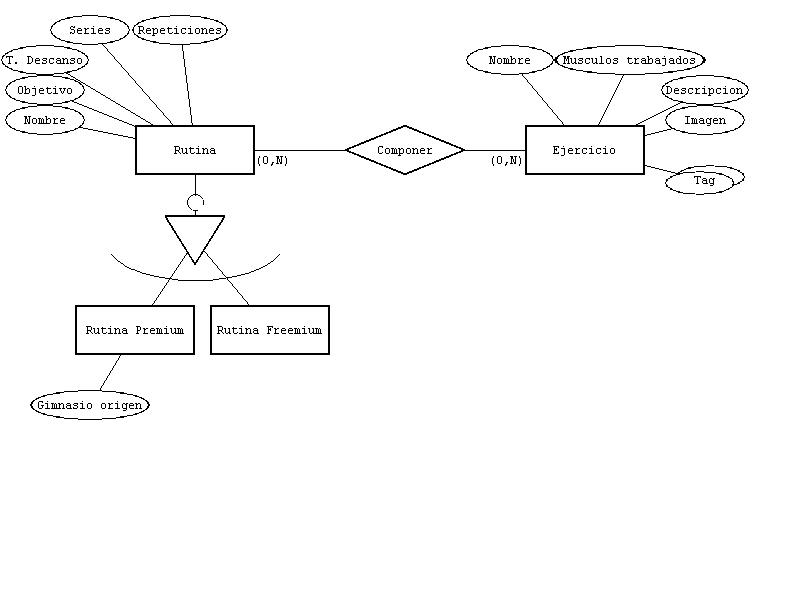
\includegraphics[width=0.7\textwidth]{capturicas/er.jpg}
	\caption{Diagrama Entidad-Relación de la BD Local}
	\label{fig: er}
\end{figure}
\subsubsection{PBI: Descarga de ejercicios}
Puntos de historia : 8
\par\textbf{Requisitos/Historias de usuario:}
\begin{itemize}
	\item El usuario debe descargar una colección de ejercicios al iniciar la aplicación, los cuales se almacenarán en la base de datos local para su visualización posterior.
	\item El usuario podrá descargar una versión actualizada de la colección de ejercicios modificada por los administradores de la aplicación.
\end{itemize}
\par\textbf{Criterios de aceptación:}
\begin{enumerate}
	\item Si no hay una BD local poblada en el dispositivo la app avisará al usuario de la
	descarga necesaria.
	\item Antes de comenzar una descarga se pide permiso al usuario sobre la descarga de archivos al teléfono móvil.
	\item Antes de comenzar una descarga se avisa al usuario del tamaño de la descarga.
	\item Se le da al usuario la opción de comenzar la descarga o salir.
\end{enumerate}
\par\textbf{Información auxiliar (bocetos GUI, documentación adicional...)}
\begin{figure}[H]
	\begin{minipage}[b]{0.5\linewidth} %Una minipágina que cubre la mitad de la página
		\begin{figure}[H]
			\centering
			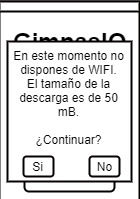
\includegraphics[width=0.5\textwidth]{capturicas/guipbidownload1.png}
			\label{fig: guipbi1}
		\end{figure}
	\end{minipage}
	\hspace{0.2cm} % Si queremos tener un poco de espacio entre las dos figuras
	\begin{minipage}[b]{0.5\linewidth}
		\begin{figure}[H]
			\centering
			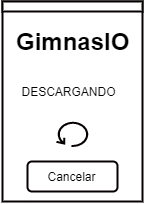
\includegraphics[width=0.5\textwidth]{capturicas/guipbidownload2.png}
			\label{fig: guipbi2}
		\end{figure}
	\end{minipage}
	\caption{Boceto GUI}
\end{figure}
\subsubsection{PBI: Ver colección de ejercicios}
Puntos de historia : 13
\par\textbf{Requisitos/Historias de usuario}
\begin{itemize}
	\item El usuario de la aplicación debe de ser capaz de poder acceder a una actividad donde se presente una lista de ejercicios almacenados en la base de datos local.
	\item Si no se ha realizado la descarga de ejercicios y la base de datos local está vacía, se mostrará una lista vacía.
	\item Si el usuario hace click en algún ejercicio, la aplicación le lleva a otra actividad dónde puede ver el ejercicio en más detalle.
\end{itemize}
\par\textbf{Criterios de aceptación}
\begin{enumerate}
	\item Se puede consultar una lista de ejercicios.
	\item Cada elemento de la lista mostrara el nombre del elemento y los tags asociados a él.
	\item Se podrá hacer clic una vez en un elemento de la lista para acceder a otra actividad con información del mismo.
\end{enumerate}
\subsubsection{PBI: Ver ejercicio}
Puntos de historia : 8
\par\textbf{Requisitos/Historias de usuario}
\begin{itemize}
	\item El usuario de la aplicación podrá ver la información de los ejercicios en detalle: su nombre, músculo utilizado, tags asociados,  imagen que describa cómo hacer el ejercicio, y una descripción que detalle cuál es la forma correcta de realizar el ejercicio.
\end{itemize}
\par\textbf{Criterios de aceptación}
\begin{enumerate}
	\item Al ver un ejercicio aparecerán entre 1 y 5 tags que clasifican el ejercicio.
	\item Al acceder al ejercicio se visualizará la imagen, músculos trabajados y descripción del mismo
\end{enumerate}
\par\textbf{Información auxiliar (bocetos GUI, documentación adicional...)}
\begin{figure}[H]
	\centering
	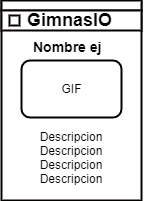
\includegraphics[width=0.2\textwidth]{capturicas/guipbiverejer.png}
	\caption{Boceto GUI}
	\label{fig: guipbi3}
\end{figure}
\subsubsection{PBI: Ver rutinas}
Puntos de historia: 8
\par\textbf{Requisitos/Historias de usuario}
\begin{itemize}
	\item El usuario de la aplicación debe de ser capaz de poder acceder a una actividad donde se presente una lista de rutinas almacenadas en la base de datos local.
	\item Si la base de datos local no almacena ninguna rutina creada por el usuario, se mostrará una lista vacía.
	\item Si el usuario hace click en una rutina de la lista, aparecerá un menú con opciones para el tratamiento de rutinas, tales como modificar, ver o eliminar.
\end{itemize}
\par\textbf{Criterios de aceptación}
\begin{enumerate}
	\item Se puede consultar una lista de rutinas.
	\item Cada elemento de la lista mostrara el nombre del elemento y el objetivo
	asociado.
	\item Se podrá hacer clic una vez en un elemento de la lista para acceder a un menú sobre el tratamiento del elemento pulsado.
\end{enumerate}
\par\textbf{Información auxiliar (bocetos GUI, documentación adicional...)}
\begin{figure}[H]
	\centering
	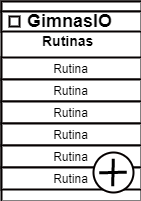
\includegraphics[width=0.2\textwidth]{capturicas/guipbiverrutinas.png}
	\caption{Boceto GUI}
	\label{fig: guipbi4}
\end{figure}
\subsubsection{PBI: Crear rutina}
Puntos de historia: 13
\par\textbf{Requisitos/Historias de usuario}
\begin{itemize}
	\item El usuario de la aplicación debe de ser capaz de poder crear una rutina, añadiendo los valores deseados a los campos de la rutina, y almacenarse en la base de datos local para su tratamiento posterior.
	\item El usuario debe ser capaz de añadir todos los ejercicios deseados a la rutina.
\end{itemize}
\par\textbf{Criterios de aceptación}
\begin{enumerate}
	\item Se puede crear una rutina y añadir ejercicios desde la lista.
	\item Al crear una rutina se permite darle un nombre, una pequeña descripción y el objetivo de dicha rutina, así como el tiempo de descanso entre ejercicios, el número de repeticiones de los ejercicios, y las series de cada ejercicio.
\end{enumerate}
\subsubsection{PBI: Ver rutina}
Puntos de historia: 8
\par\textbf{Requisitos/Historias de usuario}
\begin{itemize}
	\item El usuario de la aplicación debe de ser capaz de poder ver los campos de cada rutina en más detalle: su nombre, descripción de la misma, objetivo de la rutina, tiempo de descanso entre ejercicios, repeticiones y series de los ejercicios, y una lista de los ejercicios asignados a la rutina.
\end{itemize}
\par\textbf{Criterios de aceptación}
\begin{enumerate}
	\item Se podrá consultar una rutina una vez creada.
	\item Una vez que se está consultando la rutina se podrá acceder a cada ejercicio individualmente para consultar su información.
\end{enumerate}
\par\textbf{Información auxiliar (bocetos GUI, documentación adicional...)}
\begin{figure}[H]
	\centering
	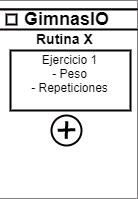
\includegraphics[width=0.2\textwidth]{capturicas/guipbiverrutina.png}
	\caption{Boceto GUI}
	\label{fig: guipbi5}
\end{figure}
\subsubsection{PBI: Modificar rutina}
Puntos de historia: 5	
\par\textbf{Requisitos/Historias de usuario}
\begin{itemize}
	\item El usuario de la aplicación puede modificar cualquier campo de la rutina deseado, incluyendo la lista de ejercicios, y guardar sus cambios  en la base de datos local.
\end{itemize}
\par\textbf{Criterios de aceptación}
\begin{enumerate}
	\item Se podrá modificar la información y todos los elementos de una rutina una vez creada.
\end{enumerate}
\subsubsection{PBI: Eliminar rutina} 
Puntos de historia: 2
\par\textbf{Requisitos/Historias de usuario}
\begin{itemize}
	\item El usuario de la aplicación puede modificar cualquier campo de la rutina deseado, incluyendo la lista de ejercicios, y guardar sus cambios  en la base de datos local.
\end{itemize}
\par\textbf{Criterios de aceptación}
\begin{enumerate}
	\item Se podrá modificar la información y todos los elementos de una rutina una vez creada.
\end{enumerate}
\subsection{Estado actual de la aplicación}
\subsubsection{Funcionalidad implementada}
En el momento actual, con el primer sprint terminado y sin contar posibles bugs encontrados, la aplicación se encuentra finalizada en su versión mas simple, donde el usuario de la aplicación puede crear rutinas personalizadas y consultar los ejercicios almacenados. Sin embargo, se ha contemplado mejoras tanto en el apartado de creación de rutinas como una mejora visual que aporte una UX mejor que la que aporta actualmente.
\subsubsection{Boceto inicial GUI}
\begin{figure}[H]
	\centering
	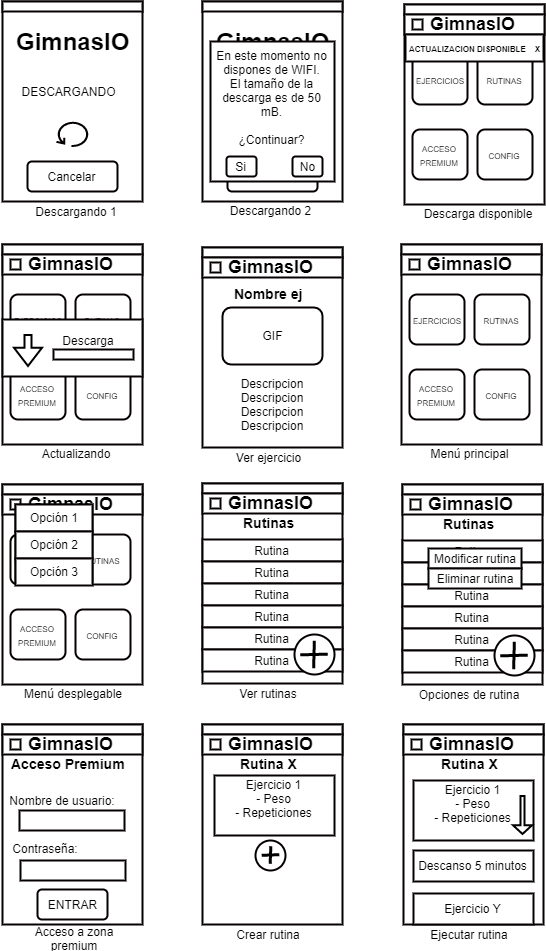
\includegraphics[width=0.6\textwidth]{capturicas/bocGui.png}
	\caption{Boceto de la GUI}
	\label{fig: bocGUI}
\end{figure}
\subsection{Aspectos de usabilidad}
\subsection{Arquitectura}
\subsubsection{Arquitectura: Servidor}
El servidor está desarrollado en \textit{Node.js} y ofrece una API Rest de la que se sirve la aplicación para las descargas y las funcionalidades online. 
\begin{figure}[H]
	\centering
	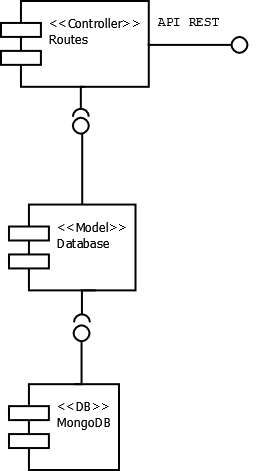
\includegraphics[width=0.2\textwidth]{capturicas/CvCSer.png}
	\caption{Diagrama CvC del Servidor}
	\label{fig: CvCSer}
\end{figure}
Este servidor ha sido desarrollado con una arquitectura por capas basada en Model-View-Controller, aunque la vista no tiene importancia en este primer sprint, por lo que no se ha representado en la \ref{fig: CvCSer}. En \ref{fig: depSer} se puede apreciar que el servidor se encuentra desplegado sobre una única máquina EC2 en la nube de Amazon Web Services. En ella se encuentran tanto la base de datos \textit{MongoDB} como la aplicación \textit{Node.js} del servidor. Desde esa máquina se ofrecen los servicios API Rest que utiliza la aplicación, que a su vez almacena los datos en su propia base de datos \textit{SQLite}.
\begin{figure}[H]
	\centering
	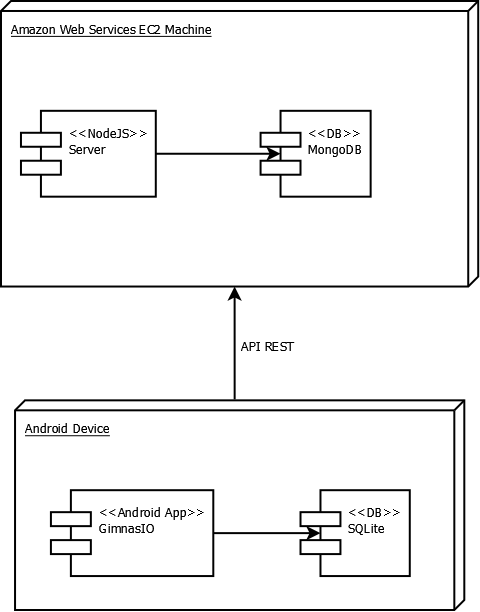
\includegraphics[width=0.7\textwidth]{capturicas/depSer.png}
	\caption{Diagrama de despliegue del servidor}
	\label{fig: depSer}
\end{figure}
La API cuenta con distintos métodos para consultar: ejercicios, rutinas, fechas de actualización, datos de almacenamiento y gimnasios registrados.
\newpage\par \textbf{Ejercicios}
\begin{figure}[H]
	\centering
	\lstinputlisting[language=python,firstline=0,lastline=23,breaklines=true,postbreak=\mbox{\textcolor{green}{$\hookrightarrow$}},xleftmargin=0.1\textwidth]{capturicas/exercisesDoc.txt}
	\caption{Especificación de la API GET \textit{/exercises/}}
	\label{cod:getExe}
\end{figure}
\begin{figure}[H]
	\centering
	\lstinputlisting[language=python,firstline=24,lastline=36,breaklines=true,postbreak=\mbox{\textcolor{green}{$\hookrightarrow$}},xleftmargin=0.1\textwidth]{capturicas/exercisesDoc.txt}
	\caption{Especificación de la API GET \textit{/exercises/download}}
	\label{cod:getDow}
\end{figure}
\newpage\par \textbf{Datos Almacenamiento}

\begin{figure}[H]
	\centering
	\lstinputlisting[language=python,breaklines=true,postbreak=\mbox{\textcolor{green}{$\hookrightarrow$}},xleftmargin=0.1\textwidth]{capturicas/dbdataDoc.txt}
	\caption{Especificación de la API GET \textit{/dbdata/}}
	\label{cod:getDbd}
\end{figure}
\par \textbf{Rutinas}
\begin{figure}[H]
	\centering
	\lstinputlisting[language=python,breaklines=true,postbreak=\mbox{\textcolor{green}{$\hookrightarrow$}},xleftmargin=0.1\textwidth]{capturicas/routinesDoc.txt}
	\caption{Especificación de la API GET \textit{/routines/}}
	\label{cod:getRou}
\end{figure}
\par \textbf{Gimnasios}
\begin{figure}[H]
	\centering
	\lstinputlisting[language=python,firstline=1,lastline=22,breaklines=true,postbreak=\mbox{\textcolor{green}{$\hookrightarrow$}},xleftmargin=0.1\textwidth]{capturicas/gymsDoc.txt}
	\caption{Especificación de la API POST \textit{/gym/newGym}}
	\label{cod:posGym}
\end{figure}
\begin{figure}[H]
	\centering
	\lstinputlisting[language=python,firstline=23,lastline=48,breaklines=true,postbreak=\mbox{\textcolor{green}{$\hookrightarrow$}},xleftmargin=0.1\textwidth]{capturicas/gymsDoc.txt}
	\caption{Especificación de la API POST \textit{/gym/newRoutine}}
	\label{cod:posRut}
\end{figure}
\par \textbf{Actualización}
\begin{figure}[H]
	\centering
	\lstinputlisting[language=python,breaklines=true,postbreak=\mbox{\textcolor{green}{$\hookrightarrow$}},xleftmargin=0.1\textwidth]{capturicas/updateDoc.txt}
	\caption{Especificación de la API GET \textit{/update/}}
	\label{cod:getDat}
\end{figure}
\subsubsection{Arquitectura: Aplicación móvil}
Para la aplicación se ha seguido la arquitectura descrita en \ref{fig: CvCApp}. El componente \textit{DBAdapter} se encarga de gestionar la base de datos ofreciendo interfaces. Para ello hace uso de los objetos de dominio que representan la información de la base de datos. Existe además un objeto \textit{JSONHandler} que se encarga de ofrecer la transformación de los objetos en formato JSON que devuelve la API a objetos en formato \textit{List}.
Finalmente, las actividades se encargan de recoger todas estas funcionalidades y utilizarlas para representar los elementos por la pantalla.
\begin{figure}[H]
	\centering
	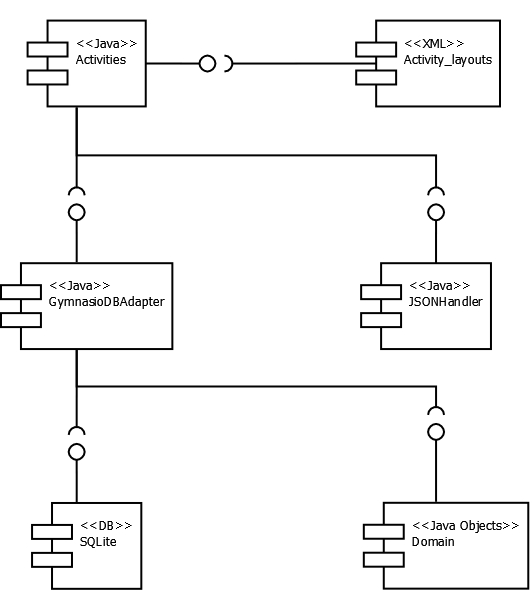
\includegraphics[width=0.7\textwidth]{capturicas/CvCApp.png}
	\caption{Diagrama CvC de la aplicación}
	\label{fig: CvCApp}
\end{figure}

\section{Segundo Sprint}
\subsection{Arquitectura}
\subsubsection{Servidor}
Se mantiene el esqueleto de la arquitectura del primer sprint, a la que se le añaden algunos componentes y se actualizan otros, de acuerdo con las necesidades de este segundo sprint.

En este segundo sprint se ha desarrollado una aplicación web implementada sobre la misma arquitectura, por lo que se ha pasado de un Modelo-Controlador donde la vista era la aplicación Android a un Modelo-Vista-Controlador completo, donde la vista es tanto la aplicación Android como la página web, siendo que los contenidos accesibles son distintos en cada una de ellas.

\begin{figure}[H]
	\centering
	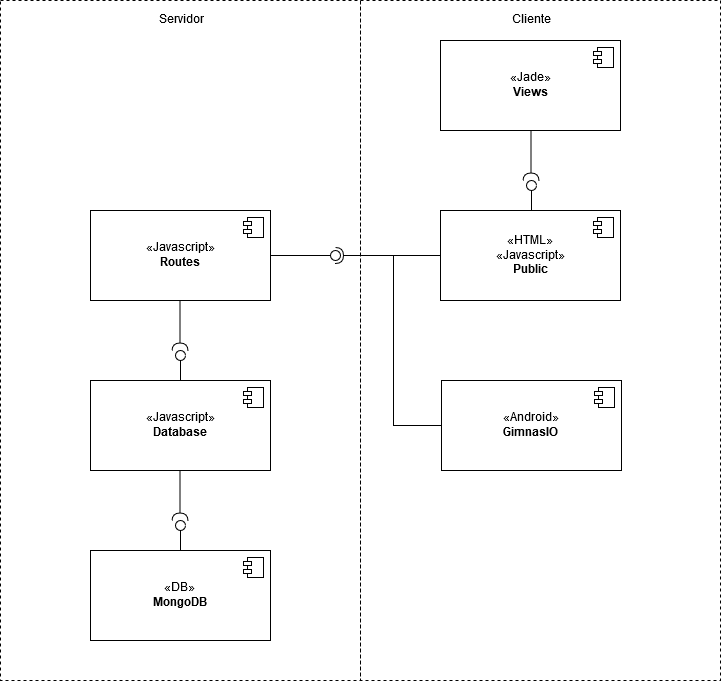
\includegraphics[width=0.7\textwidth]{graficos/CyCserver.png}
	\caption{Diagrama CyC del servidor }
	\label{fig: CyCServ2}
\end{figure}
Se mantiene la API Rest como método de comunicación del servidor con el exterior. En la parte de Cliente, la aplicación Android accede a la API Rest de forma nativa con librerías Java, mientras que para la web, se ha utilizado Javascript (jQuery) y Ajax para realizar las peticiones y controlar los contenidos de las páginas estáticas.


Además, se han realizado algunas modificaciones y añadido funcionalidades a la API existente. Estas son:
\begin{itemize}
	\item Pedir rutinas: Modificada para no devolver repeticiones, series y tiempo de descanso para cada rutina, sino que esa información esté contenida en cada ejercicio.

	\item Actualizar rutina: Nueva entrada para permitir modificar repeticiones, series y tiempo de descanso para cada ejercicio.

	\item Nueva rutina: Nueva entrada para permitir establecer repeticiones, series y tiempo de descanso para cada ejercicio.

	\item Borrar rutina: Nueva entrada utilizada para borrar rutinas en el servidor.

	\item Nuevo gimnasio: Modificada para enviar las claves por email en vez de en la respuesta.

	\item Login gimnasio: Nueva entrada utilizada para comprobar las credenciales de entrada a la parte premium. Devuelve si son correctos o no, y en caso afirmativo, el tipo de usuario.

	\item Pedir ejercicios: Modificada para permitir devolver repeticiones, series y tiempo de descanso para cada ejercicio.

\end{itemize}
\begin{figure}[H]
	\centering
	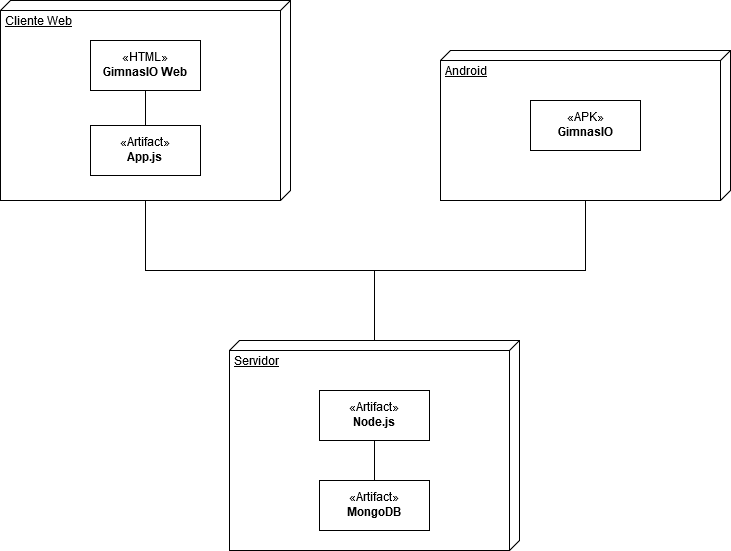
\includegraphics[width=0.8\textwidth]{graficos/despliegue.png}
	\caption{Diagrama de Despliegue }
	\label{fig: deploy2}
\end{figure}
\begin{figure}[H]
	\centering
	\lstinputlisting[breaklines=true,postbreak=\mbox{\textcolor{green}{$\hookrightarrow$}},xleftmargin=0.1\textwidth]{files/gyms.txt}
	\caption{Especificación de la API gym}
	\label{cod:apiEx}
\end{figure}
\begin{figure}[H]
	\centering
	\lstinputlisting[breaklines=true,postbreak=\mbox{\textcolor{green}{$\hookrightarrow$}},xleftmargin=0.1\textwidth]{files/exercises.txt}
	\caption{Especificación de la API exercises}
	\label{cod:apiRou}
\end{figure}
\newpage
\begin{figure}[H]
	\centering
	\lstinputlisting[breaklines=true,firstline=0,lastline=50,postbreak=\mbox{\textcolor{green}{$\hookrightarrow$}},xleftmargin=0.1\textwidth]{files/routines.txt}
	\label{cod:apiGym}
\end{figure}
\begin{figure}[H]
	\centering
	\lstinputlisting[breaklines=true,firstline=51,postbreak=\mbox{\textcolor{green}{$\hookrightarrow$}},xleftmargin=0.1\textwidth]{files/routines.txt}
	\caption{Especificación de la API routines}
	\label{cod:apiGym}
\end{figure}
\subsubsection{Aplicación móvil}
Se mantiene una vez más el esqueleto de la arquitectura del primer sprint. Sin embargo, en este sprint se han realizado esfuerzos para modularizar el código y permitir una mayor reusabilidad de métodos y objetos. 

\begin{figure}[H]
	\centering
	\includegraphics[width=0.7\textwidth]{graficos/CyCApp.png}
	\caption{Diagrama CyC de la aplicación }
	\label{fig: CyCApp2}
\end{figure}
Se pueden observar dos nuevos componentes \textit{Services} y \textit{Database}, uno completamente nuevo y el otro toma el lugar de \verb|GymnasioDBAdapter|. Ambos son fruto de dicho proceso de modularización del código. Database contiene todos los objetos y métodos que interactúan con la base de datos SQLite. Por otro lado, Services representa los métodos encargados de interactuar con APIs externas, que en este caso es el servidor de GimnasIO.


\chapter{Proceso}
\section{Primer Sprint}
\subsection{Estrategia y herramientas en test y cobertura de código}
Se ha seguido la estrategia de crear como mínimo un test unitario por función de la aplicación que no se base en la interacción con el usuario. Por lo tanto se han testeado acciones como operaciones de acceso a la base de datos local y peticiones a la base de datos remota, pero no se han testeado el correcto funcionamiento de los botones o demás elementos interactuables de la aplicación. Los test que incluyan interacción con el usuario serán realizados en una etapa posterior del proyecto, cuando el diseño de las GUI este más cerca de ser el definitivo. %Estos test de elementos interactivos se realizaran mediante la librería Espresso, la cual permite simular acciones que podrían ser llevadas por un usuario real utilizando la aplicación.

Para testear la aplicación se ha utilizado la librería JUnit, la cual permite la creación de test de una manera rápida y sencilla. Además es la librería con la que más miembros del equipo habían trabajado, por lo que se consideró la mejor opción.

Por tanto en este sprint se han testeado las operaciones en la base de datos local y las peticiones al servidor remoto, consiguiendo un cobertura del 82\% para el servidor remoto. La cobertura de la aplicación no se puede calcular debido a los problemas de integración con \textit{Travis CI}.

\subsection{Estrategia para la construcción automática de software}
Debido a que el equipo utiliza Github como herramienta de control de versiones, se ha decidido aprovechar algunas de las herramientas de integración continua que son aplicables a Github. Se planteó desde el principio añadir \textit{Travis CI} a los dos repositorios Github del equipo (el de la aplicación y el del servidor remoto) para que cada vez que hubiera una actualización de código en el repositorio, \textit{Travis CI} pasara todos los tests para comprobar si el nuevo codigo era correcto. 

Se ha conseguido añadir \textit{Travis CI} al repositorio del servidor remoto de forma satisfactoria, pero no se ha conseguido añadir al repositorio de la aplicación. El equipo ha empleado muchas horas en este intento sin obtener ningún resultado correcto, por tanto se esta planteando la posibilidad de utilizar en el repositorio de la aplicación una herramienta distinta a Travis. Actualmente el equipo esta explorando alternativas a dicha herramienta.
\subsection{Definición de hecho}
Se ha tomado la decisión de que una tarea estará completa cuando cumpla la definición de hecho, que está conformada por los siguientes puntos:
\begin{itemize}
	\item Todas las tareas de una entrada de la pila están completadas.
	\item Se han escrito y ejecutado test unitarios con al menos un $50\%$ de cobertura como resultado.
	\item Se ha comprobado que, al terminar las tareas de una entrada, el resto de test siguen dando un resultado satisfactorio.
	\item Se ha realizado una documentación de mínimos del diseño e implementación del código de cara a entender el funcionamiento de este, mediante especificaciones en el código y diagramas de diseño e implementación.
	\item Se ha probado su correcto funcionamiento en dos dispositivos Android diferentes: OnePlus One y Nexus 4 emulado. Se prueba en el emulador durante el desarrollo y en el dispositivo físico una vez finalizadas las tareas. Se probará tanto de manera automática corriendo los test, como de manera manual, utilizando las funcionalidades recién implementadas.
\end{itemize}
\subsection{Estrategia de control de versiones}
Para el control de versiones se ha creado una organización como se indicaba desde el profesorado de la asignatura, ademas dado que el proyecto se divide en dos entornos, el primero de ellos la propia aplicación Android y el segundo el servidor que provee los datos de ejercicios se decidió que se dividiría en dos repositorios independientes para evitar problemas entre ellos, sobre esos repositorios se estableció una política basada en forks donde cada miembro del equipo realizaba un fork del repositorio principal y actualiza el repositorio principal tras la finalización de un \textit{issue} mediante un pull request que previa a su aceptación debe ser revisado por otro miembro, estableciendo un \textit{pseudo-responsable} de cada subrepositorio, que en caso de duda es el responsable último de la decisión de aceptación.
\subsection{Esfuerzos por persona}
\begin{figure}[H]
	\centering
	\begin{tikzpicture}
	\begin{axis}[
	ybar,
	enlargelimits=0.15,
	legend style={at={(0.5,-0.2)},
		anchor=north,legend columns=-1},
	ylabel=Horas Invertidas,
	symbolic x coords={Alberto, Alejandro, Asier, Darío},
	xtick=data,
	nodes near coords, 
	nodes near coords align={vertical},
	x tick label style={rotate=45,anchor=east},
	]
	\addplot coordinates {(Alberto,65) (Alejandro,44) 
		(Asier,60) (Darío,50)};
	\end{axis}
	\end{tikzpicture}
	\caption{Distribución de horas invertidas en el primer Sprint.}
\end{figure}
\subsection{Diagrama de trabajo completado/pendiente}
\subsection{Velocidad del equipo}
A continuación en \ref{fig: burup} y \ref{fig: burdow} se muestran la gráfica de seguimiento del sprint:
\begin{figure}[H]
	\centering
	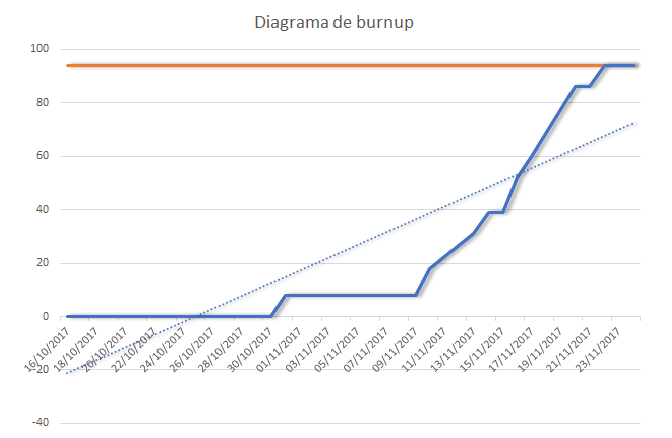
\includegraphics[width=0.7\textwidth]{capturicas/burnup.png}
	\caption{Diagrama Burnup}
	\label{fig: burup}
\end{figure}
\begin{figure}[H]
\centering
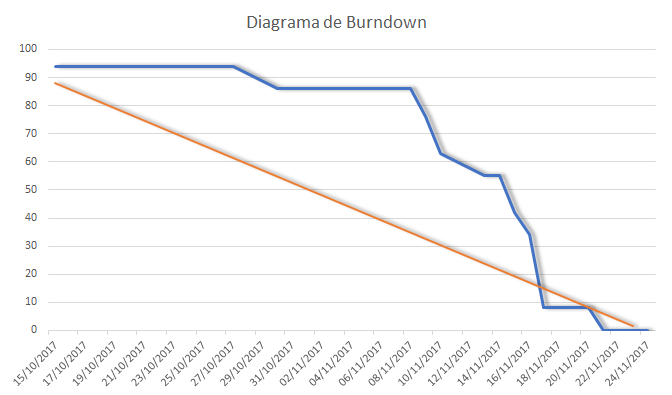
\includegraphics[width=0.7\textwidth]{capturicas/burndown.png}
\caption{Diagrama Burndown}
\label{fig: burdow}
\end{figure}
La velocidad del equipo ha sido de 94 P.H en este sprint.
\subsection{Resultados de la última retrospectiva}
En la reunión de retrospectiva con el profesorado se han extraído varias conclusiones:
\begin{itemize}
	\item La escasa modularización del código ha dificultado el testeo.
	\item No se ha podido determinar la cobertura de código de la aplicación.
	\item Se necesitó reescribir el código de la base de datos local.
	\item Documentación de la API poco definida provoco confusiones en la implementación de la misma.
	\item Algunos miembros del equipo fueron reacios a modificar código ajeno a sus tareas.
	\item Una mala estimación de las PBI provocó que una entrada de la pila llegara al sprint demasiado grande y que fuera necesario fraccionarla y reestimarla.
	\item La falta de formación en el entorno Android afecto negativamente al tiempo y a las estimaciones.
	\item En algunos momentos del sprint el \textit{Work in Progress} era demasiado alto.
	\item Desuso del tablero Scrum.
	\item No se consiguió integrar \textit{Travis CI} con Android.
\end{itemize}
Tras una puesta en común entre los miembros del equipo de los problemas encontrados se ha determinado los tres problemas mas prioritarios a resolver en el siguiente sprint:
\begin{itemize}
	\item \textbf{Modularización del código:} 
	\\Se van a aplicar patrones Vista-Controlador para el desarrollo de las funcionalidades.
	\\Se ha decidido crear una PBI para solucionar este problema.
	\item \textbf{Desuso del tablero Scrum:}
	\\El ScrumMaster revisara el tablero al menos una vez a la semana supervisando que el tablero refleja la situación actual del equipo.
	\item \textbf{Integración de \textit{Travis CI} con Android:}
	\\Se ha decidido buscar una herramienta alternativa a \textit{Travis CI}.
	\\Se creará una PBI para solucionar este problema.
\end{itemize}
\subsection{Otros aspectos de la gestión de proyecto y/o proceso de trabajo}
\begin{figure}[H]
	\centering
	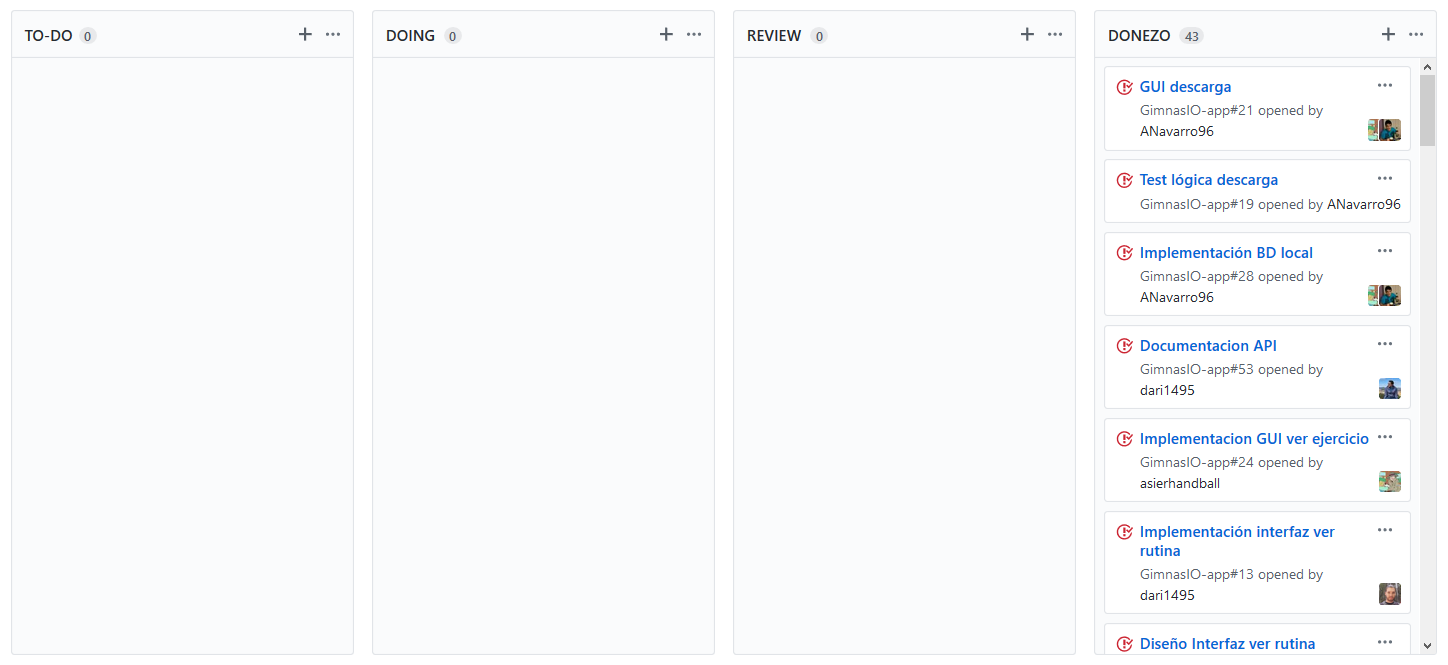
\includegraphics[width=0.7\textwidth]{capturicas/tablerico.png}
	\caption{Tablero}
	\label{fig: tablero}
\end{figure}
Para la gestión del tablero del sprint se ha utilizado la herramienta de Github Projects. Para ello, se ha creado un proyecto en el perfil de la organización en el que se manejarán las tareas en un tablero formado por cuatro columnas:
\begin{itemize}
	\item \textbf{TO-DO:} Es la columna de tareas que no se están realizando en este momento
	\item \textbf{DOING:} Tareas que actualmente se están desarrollando.
	\item \textbf{REVIEW:} Tareas que se han enviado en un PR para la aprobación del equipo. Una vez aprobadas, esas tareas se considerarán hechas. Este tablero, junto a DOING, representa el WiP del equipo.
	\item \textbf{DONE:} Tareas terminadas.
\end{itemize}
En el tablero se representan las tareas como tarjetas interactivas. Cada una de estas tarjetas es, en realidad, un Issue creado en uno de los repositorios de la organización. Esto nos permite sacar el máximo partido a la herramienta de Github projects, y es uno de los motivos por los que se eligió frente a las otras posibilidades. Esta herramienta nos permite además crear Milestones en la misma pestaña Issues. Una Milestone representa un objetivo, y por tanto se le puede añadir una fecha de finalización y asignarle Issues previamente creados. Resulta entonces una herramienta perfecta para representar las entradas de la pila, con la fecha de finalización del sprint como objetivo y una serie de Issues que representan cada tarea de la entrada de la pila asignadas a ese Milestone. Además, conforme se van cerrando los Issues asignados a una Milestone, se puede ver el porcentaje de tareas completadas, aportando de esta manera un feedback visual que permite ver de un vistazo cuánto falta para finalizar cada entrada de la pila.
El workflow deseado con esta implementación es tal que:
\begin{itemize}
	\item Una o más personas se asignan una tarea de la columna TO-DO utilizando la herramienta Issues de Github.
	\item El o los encargados de esa tarea la mueven a la columna DOING cuando empiecen a trabajar en ella.
	\item Cuando consideran que está hecha, mandan un Pull Request al repositorio principal y la mueven a la columna REVIEW. El Pull Request cuenta en la descripción con una referencia a la Issue de la tarea completada. (P.Ej.: Cerrado issue \#21)
\end{itemize}
Aquí se producen dos escenarios posibles:
\begin{itemize}
\item El Pull Request es aceptado, de forma que la tarea se cierra automáticamente gracias a la referencia. La tarjeta se mueve definitivamente a la columna DONE.
\item El Pull Request es incorrecto, incompleto o incompatible con el contenido del repositorio. En ese caso, la tarjeta se mueve de vuelta a la columna DOING hasta que se esté listo para volverlo a enviar.
\end{itemize}
De esta forma, un vistazo al tablero permite ver el WiP actual, las tareas que quedan por realizar e incluso si hay algún Pull Request pendiente de aprobación.
En este primer sprint este workflow ha sido ligeramente deficiente en la práctica. El alto requerimiento de atención que exige para mantenerse actualizado provoca que por un despiste de algún miembro del equipo el tablero se desactualice y pierda precisión, pudiendo provocar duplicidades de trabajo o confusión generalizada. El problema se produce cuando estos despistes se convierten en algo habitual, cosa que, por suerte, no ha llegado a ser realmente grave.
De cara al segundo sprint se pretende realizar un énfasis en esta implementación. Los miembros del equipo serán recordados al menos una vez a la semana de mantener actualizadas sus tareas en el tablero, y, a su vez, se les exigirá una mayor atención hacia el tablero.
\section{Segundo Sprint}
\subsection{Estrategia y herramientas en test y cobertura de código}
En este segundo sprint se ha seguido con la misma dinámica de tests que se llevó en el primer sprint. Por ello, se han creado los tests unitarios correspondientes a las entradas de pila realizadas en el segundo sprint. Además, se han añadido tests de aceptación automatizados para testear la GUI, los cuales no pudieron hacerse durante el primer sprint ya que en ese momento la GUI estaba lejos de ser la definitiva. La API web también ha sido completada con algunos tests para cubrir las funcionalidades implementadas en este segundo sprint.


\subsubsection{Test unitarios de la base de datos}

Tras este segundo sprint, la colección de tests unitarios para la interacción con la base de datos local contiene los siguientes tests:

\paragraph{Tests sobre ejercicios:}
\begin{itemize}
	\item \textit{addExerciseTest()}: comprueba que se añaden correctamente ejercicios a la base de datos.

	\item \textit{addExerciseTestRepeated()}: comprueba que no se añade un ejercicio a la base de datos si este ya se encuentra en la misma.

	\item \textit{deleteExerciseTest()}: comprueba que la base de datos borra correctamente un ejercicio contenido en ella.

	\item \textit{dontDeleteExerciseTest()}: comprueba que la base de datos se comporta correctamente cuando se intenta eliminar un ejercicio no contenido en ella.

	\item \textit{checkExerciseByName()}: comprueba que la base de datos devuelve correctamente la información de todos los ejercicios contenidos en ella cuyos campos “nombre” son o contienen el nombre buscado.

	\item \textit{checkExerciseByNameFalse()}: comprueba que la base de datos no devuelve nada cuando ningún ejercicio contenido en ella tiene un campo “nombre” que sea o contenga el nombre buscado.

	\item \textit{checkExerciseByMuscle()}: comprueba que la base de datos devuelve correctamente la información de todos los ejercicios contenidos en ella cuyos campos “músculo” son o contienen el músculo buscado.

	\item \textit{checkExerciseByMuscleFalse()}: comprueba que la base de datos no devuelve nada cuando ningún ejercicio contenido en ella tiene un campo “músculo” que sea o contenga el músculo buscado.

	\item \textit{checkExerciseByTag()}: comprueba que la base de datos devuelve correctamente la información de todos los ejercicios contenidos en ella cuyos campos “tag” son o contienen el tag buscado.

	\item \textit{checkExerciseByTagFalse()}: comprueba que la base de datos no devuelve nada cuando ningún ejercicio contenido en ella tiene un campo “tag” que sea o contenga el tag buscado.

\end{itemize}
\paragraph{Tests sobre rutinas:}
\begin{itemize}
	\item \textit{addFreemiumRoutineTest()}: comprueba que se inserta correctamente una rutina de tipo “freemium” en la base de datos.

	\item \textit{addPremiumRoutineTest()}: comprueba que se inserta correctamente una rutina de tipo “premium” en la base de datos.

	\item \textit{getFreemiumRoutineTest()}: comprueba que la base de datos devuelve correctamente la información de una rutina almacenada en ella al buscarla por su “id”.

	\item \textit{deleteRoutineTest\_existe()}: comprueba que la base de datos elimina correctamente una rutina almacenada en ella al introducir su “id”.

	\item \textit{deleteRoutineTest\_cero()}: comprueba que la base de datos se comporta correctamente (ni elimina ni falla) cuando se intenta eliminar una rutina con “id” cero.

	\item \textit{deleteRoutineTest\_negativo()}: comprueba que la base de datos se comporta correctamente (ni elimina ni falla) cuando se intenta eliminar una rutina con “id” negativo.

	\item \textit{updateNameRoutineFreemium()}: comprueba que el valor del campo “nombre” de una rutina freemium se actualiza correctamente en la base de datos cuando es modificado.

	\item \textit{updateNameGymRoutineFreemium()}: comprueba que el valor del campo “gym” de una rutina freemium se actualiza correctamente en la base de datos cuando es modificado.

	\item \textit{updateObjRoutineFreemium()}: comprueba que el valor del campo “objetivo” de una rutina freemium se actualiza correctamente en la base de datos cuando es modificado.

	\item \textit{updateExsRoutineFreemium()}: comprueba que los ejercicios asignados a una rutina freemium se actualizan correctamente en la base de datos cuando son modificados.

	\item \textit{fetchAllPremiumRoutinesTest()}: comprueba que la base de datos devuelve correctamente todas las rutinas premium almacenadas en la base de datos local.

	\item \textit{getNumberOfRoutinesTest()}: comprueba que la función de la base de datos que devuelve el número total de rutinas almacenadas devuelve el número correcto.

	\item \textit{getRoutineByNameTest()}: comprueba que la base de datos devuelve correctamente la información de las rutinas almacenadas en ella cuyos campos “nombre” sean o coincidan con el nombre buscado.

	\item \textit{dontGetRoutineByNameTest()}: comprueba que la base de datos no devuelve nada cuando ninguna rutina almacenada en ella tiene un campo “nombre” que sea o contenga el nombre buscado.

	\item \textit{getRoutineByObjectiveTest()}: comprueba que la base de datos devuelve correctamente la información de las rutinas almacenadas en ella cuyos campos “objetivo” sean o coincidan con el objetivo buscado.

	\item \textit{dontGetRoutineByObjectiveTest()}: comprueba que la base de datos no devuelve nada cuando ninguna rutina almacenada en ella tiene un campo “objetivo” que sea o contenga el objetivo buscado.

\end{itemize}

\subsubsection{Test de llamadas a la api remota}

En este segundo sprint, tras implementar la parte premium de la aplicación se han diseñado una serie de test de interacción con el servidor remoto para comprobar el correcto funcionamiento de las llamadas a la API. Los tests implementados han sido los siguientes:

\begin{itemize}
	\item \textit{loginPremium\_Test()}: comprueba que la petición de login al servidor remoto funciona correctamente.

	\item \textit{dbData\_Test()}: comprueba que la petición para obtener la información de la base de datos remota (tamaño del contenido de los ejercicios para descargar) funciona correctamente.

	\item \textit{updateDb\_Test()}: comprueba que la petición para actualizar la base de datos local con los ejercicios contenidos de la base de datos remota funciona correctamente.

	\item \textit{updatePremiumDb\_Test()}: comprueba que la petición para descargar las rutinas premium de un gimnasio almacenadas en la base de datos remota funciona correctamente.

	\item \textit{downloadImg\_Test()}: comprueba que la peticion para descargar la imagen asociada a un ejercicio almacenado en la base de datos remota funciona correctamente.

	\item \textit{createPremiumRoutine\_Test()}: comprueba que las peticiones para crear, modificar y eliminar rutinas premium en la base de datos remota funciona correctamente.

\end{itemize}
\subsubsection{Test de aceptación automáticos}
En este sprint se han añadido una serie de test de aceptación automáticos para comprobar que todas las funcionalidades de la aplicación funcionan correctamente al usar la aplicación. Para ello se ha testeado la GUI de la aplicación con la herramienta de automatización Espresso. Los tests creados han sido los siguientes:

\begin{itemize}
	\item \textit{testVerEjercicios()}: comprueba que la pantalla de ver ejercicios es alcanzable desde la interfaz de la aplicación.

	\item \textit{testVerEjercicio()}: comprueba que la pantalla de ver la información de un ejercicio es alcanzable desde la interfaz de la aplicación.

	\item \textit{testVerRutinas()}: comprueba que la pantalla de ver la lista de rutinas freemium es alcanzable desde la interfaz de la aplicación.

	\item \textit{testCrearModificarEliminarRutinaFreemium()}: comprueba que es posible crear, modificar y eliminar una rutina freemium desde la interfaz de la aplicación.

	\item \textit{testLoginPremiumAsNormalUserAndLogout()}: comprueba que el inicio de sesión como usuario premium normal, así como el cerrado de la sesión abierta, funcionan correctamente desde la interfaz de la aplicación.

	\item \textit{testLoginPremiumAsTrainerUserAndLogout()}: comprueba que el inicio de sesión como usuario premium entrenador, así como el cerrado de la sesión abierta, funcionan correctamente desde la interfaz de la aplicación.

	\item \textit{testCrearModificarEliminarRutinaPremium()}: comprueba que es posible crear, modificar y eliminar una rutina premium desde la interfaz de la aplicación.

	\item \textit{testModificarEjerciciosDentroDeRutina()}: comprueba que es posible modificar los atributos de un ejercicio añadido a una rutina desde la interfaz de la aplicación.

	\item \textit{testMoverEjerciciosDentroDeRutina()}: comprueba que es posible modificar la posición que tiene  un ejercicio añadido a una rutina dentro de la misma desde la interfaz de la aplicación.
\end{itemize}
\subsection{Estrategia para la construcción automática de software}
Se mantiene la configuración del servidor que construye, realiza las pruebas e informa del coverage del anterior sprint.

Una de las tareas de este segundo sprint era la de buscar una herramienta alternativa a Travis que permitiese ejecutar las pruebas en Android. Tras una ardua investigación y horas de infructuoso trabajo, se decide que ninguna alternativa cumple nuestras expectativas, y, por tanto, se decide volver a Travis y abandonar la idea de probar los test de integración automáticamente. En su lugar se realiza únicamente la construcción del proyecto. Sin embargo, en el afán de realizar algo más allá de la construcción, se implementa en Travis que se genere una reléase en Github por cada versión pusheada. Esta implementación se realiza en uno de los repositorios personales (@dari1495 \url{https://github.com/dari1495/GimnasIO-app/releases} ]) .
\subsection{Definición de hecho}
\subsection{Estrategia de control de versiones}
Se mantiene la división en dos repositorios del primer sprint, uno para la aplicación Android y otro para el servidor web. 

\begin{figure}[H]
	\centering
	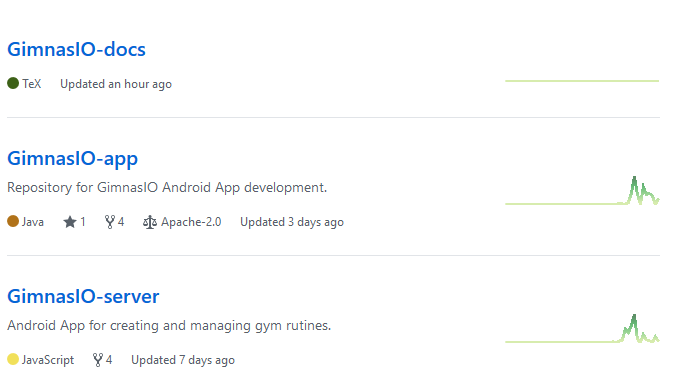
\includegraphics[width=1\textwidth]{graficos/repos.png}
	\caption{Repositorios del proyecto.}
	\label{fig: repos}
\end{figure}
La única novedad de este sprint es la creación de un nuevo repositorio únicamente para documentación llamado GimnasIO-docs. En este repositorio se somete a control de versiones la documentación del sistema. Este repositorio no se somete a un control tan exhaustivo de versiones, permitiendo a los miembros del equipo pushear contenido sin revisión previa.

\subsection{Esfuerzos por persona}
\begin{figure}[H]
	\centering
	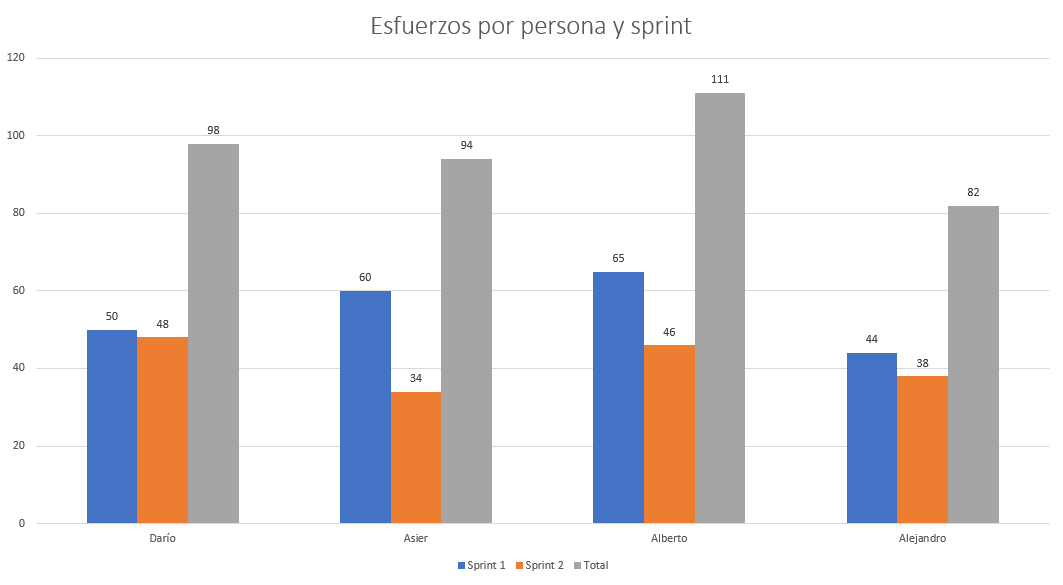
\includegraphics[width=1\textwidth]{graficos/esfuerzos.png}
	\caption{Repositorios del proyecto.}
	\label{fig: repos}
\end{figure}
Se puede observar un reparto más o menos parecido de los esfuerzos por persona, cumpliendo el mínimo aproximado de 90h de esfuerzo en la asignatura. Lo más destacable es, probablemente, que haya una menor cantidad de horas trabajadas este segundo sprint pese a haber realizado más puntos de historia. Esto puede ser debido a la experiencia ganada en el primer sprint en cuanto a las tecnologías utilizadas y el trabajo en equipo.

\subsection{Velocidad del equipo}
Este segundo sprint se prestó más atención a la metodología de trabajo, especialmente a uno de los mayores problemas del primer sprint que fue la acumulación de WIP (Work In Progress). La velocidad del equipo en este Sprint ha sido de 119 P.H.

Siguiendo el diagrama de burnup, el comienzo del sprint sigue sin aparentar mejoría, pero realmente es debido a la existencia de entradas de la pila “bloqueantes” que impedían cerrar otras entradas hasta que las primeras no fueran terminadas. Se observa una clara mejoría una vez superados los “baches” de las entradas bloqueantes.
 
\begin{figure}[H]
 
	\centering
 
	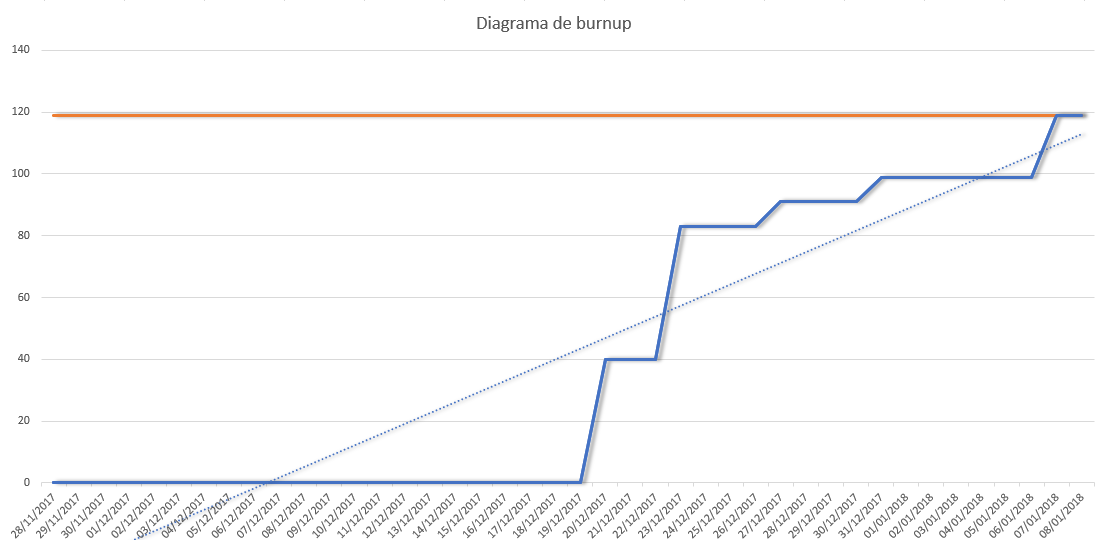
\includegraphics[width=1\textwidth]{graficos/burnup.png}
 
	\caption{Diagrama de Burnup.}
 
	\label{fig: burnup2}
 
\end{figure}

La mejoría es mucho mas evidente si se observa el diagrama de burndown, donde se utilizan las horas de coste para cada tarea cerrada como métrica en lugar de puntos de historia. Se observa que, salvo al principio del sprint, se trabaja siempre por debajo del ritmo normal, con lo que se demuestra el ritmo constante de trabajo que no se refleja en el diagrama de burnup.

\begin{figure}[H]
	\centering
	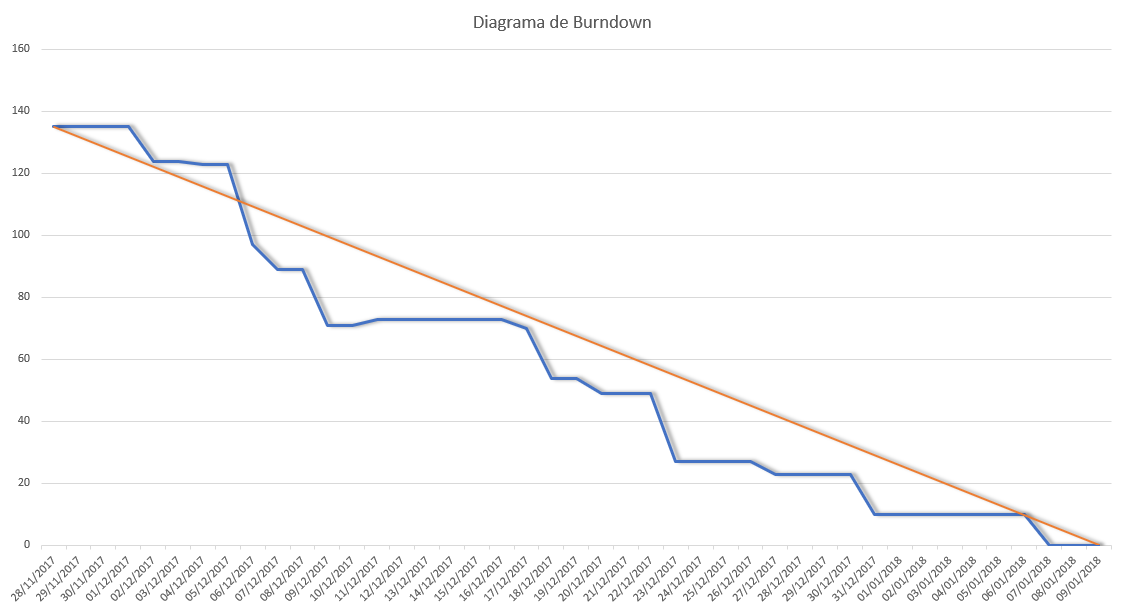
\includegraphics[width=1\textwidth]{graficos/burndown.png}
	\caption{Diagrama de Burndown.}
	\label{fig: burndown2}
\end{figure}
\chapter{Conclusiones}
\section{Primer Sprint}
Se espera obtener un grado de al menos notable en este primer sprint. Para ello se han seguido las recomendaciones establecidas en la presentación de Evaluación del proyecto. Las conseguidas satisfactoriamente son:
\begin{itemize}
	\item \textbf{El código del proyecto se aloja en Github y se trabaja de forma habitual contra él.} El equipo ha trabajado continuamente contra dos repositorios de Github.
	\item \textbf{El software funciona correctamente e implementa suficiente funcionalidad.} La app al final del primer sprint implementa correctamente las funcionalidades propuestas para este sprint.
	\item \textbf{Informe de proyecto suficiente y adecuado.} En este mismo documento se encuentran todas las secciones demandadas, así como la documentación del diseño y la implementación del sistema.
	\item \textbf{Cobertura de tests automáticos de al menos el 30\% del código.} El servidor tiene una cobertura del 82\% del código, esto se puede consultar en el repositorio del servidor en la medalla de Codecov presente en el readme.Pese a que no conocemos aún la cobertura del código Android, con la cantidad de test que ahora mismo se encuentran programados, es seguro decir que esa cobertura es perfectamente alcanzable. Se espera mejorar en el segundo sprint hacia más de un 50% de cobertura.
	\item \textbf{Al menos el 50\% de las historias de usuario / requisitos tienen buenos criterios de aceptación.} Se ha trabajado de forma que todos los requisitos tengan buenos criterios de aceptación.
	\item \textbf{Definición de hecho clara.} La definición de hecho existente al final del primer sprint se considera suficientemente clara, pese a que de cara al segundo sprint se van a plantear algunas mejoras.
	\item \textbf{Compilación y gestión de dependencias.} A nivel de servidor, se ha utilizado npm para la gestión de dependencias y lanzamiento. A nivel de aplicación, se ha utilizado Gradle.
	\item \textbf{Se lleva un control de esfuerzos con horas dedicadas por persona a cada tarea.} Se han entregado ya distintas hojas de esfuerzos con el desglose por persona de las horas dedicadas y a que tareas.
	\item \textbf{Toda la documentación del proyecto está bajo control de versiones.} La documentación del proyecto se encuentra en el Dropbox del equipo, por lo que se considera que la gestión de versiones de este sistema es suficiente para esta tarea.
\end{itemize}
Además, se han realizado algunas de las tareas del sobresaliente:
\begin{itemize}
	\item \textbf{Todas las historias de usuario / requisitos implementados tienen buenos criterios de aceptación.} Como se ha mencionado anteriormente, todos los requisitos del proyecto están dotados de buenos criterios de aceptación.
	\item \textbf{La construcción se ha automatizado más allá de la compilación y gestión de dependencias.} Este requisito se ha completado a medias, en la parte de servidor, la integración con TravisCI y Codecov permite no solo construir el código y sus dependencias, sino comprobar el funcionamiento de los test y realizar un informe incluyendo la cobertura de código. En el segundo sprint se trabajará para implementar esta funcionalidad también en el proyecto de la aplicación y ampliarla hacia la generación del APK automáticamente y el despliegue automático del servidor cuando haya cambios en el repositorio.
\end{itemize}
\section{Segundo Sprint}
Se espera obtener un grado de sobresaliente en este segundo sprint. Para ello se han cumplido los requisitos establecidos en la presentación de Evaluación del proyecto. Estas son:
\begin{itemize}
	\item 	\textbf{El código del proyecto se aloja en Github y se trabaja de forma habitual contra él.} El equipo ha trabajado continuamente contra tres repositorios de Github.
	\item \textbf{El software funciona correctamente e implementa suficiente funcionalidad.} La aplicación contiene todas las funcionalidades acordadas e incluso se dispone de una aplicación Web para las funcionalidades externas a ella.

	\item \textbf{Informe de proyecto suficiente y adecuado.} En este documento se encuentran todas las secciones demandadas, así como la documentación de diseño e implementación del sistema y el manual de usuario.

	\item \textbf{Cobertura de test automáticos de al menos 50\% del código.} El servidor tiene una cobertura de 81\% de código \url{https://codecov.io/gh/UNIZAR-30248-2017-GIMNASIO/GimnasIO-server}. La cobertura en Android, debido al tipo de test utilizado, ha resultado imposible de obtener. Sin embargo, como se testearon todas las funcionalidades, es seguro decir que el 50\% de cobertura es perfectamente alcanzable.

	\item \textbf{Definición de hecho clara.} La definición de hecho revisada y corregida de este segundo sprint se considera suficiente para satisfacer este requisito.

	\item \textbf{Compilación y gestión de dependencias.} A nivel de servidor, se ha utilizado npm. A nivel de aplicación, se ha utilizado Gradle.

	\item \textbf{Toda la documentación está bajo control de versiones. }Toda la documentación se encuentra tanto en Dropbox como en un repositorio de Github creado específicamente a tal efecto llamado gimnasio-docs.

	\item \textbf{Todas las historias de usuario tienen buenos criterios de aceptación.} Los expuestos en este documento se consideran suficientemente buenos para ello.

	\item \textbf{Se lleva un control de esfuerzos con horas dedicadas por persona a cada tarea.} Se han realizado todas las entregas de la hoja de esfuerzos con el desglose por persona de las horas dedicadas y a que tareas.

	\item \textbf{La construcción se ha automatizado mas allá de la compilación y gestión de dependencias.} En la parte del servidor, con la implementación de Travis y Codecov se genera de forma automática un reporte de la cobertura de código. En el lado de Android, se genera de forma automática una reléase de Github a través también de Travis.

\end{itemize}
\chapter{ANEXO I: MANUAL DE USUARIO}
\section{Información general}
GimnasIO es una aplicación para Android diseñada y desarrollada por cuatro alumnos de la Universidad de Zaragoza. La aplicación se ha creado para ayudar a usuarios de gimnasios a poder organizar sus rutinas; la aplicación les ofrece una lista de ejercicios, y les permite crear rutinas en local, seleccionado los ejercicios, las repeticiones, series y tiempo de descanso de cada ejercicio. La aplicación le da la opción al usuario de ejecutar la rutina, es decir, que automática prepara un contador de tiempo para que el usuario pueda navegar entre los diversos ejercicios de la rutina y pueda controlar el tiempo de descanso, o el tiempo que tarda en hacer sus ejercicios.

Además, también se ha incluido una versión de pago, en la que los diversos gimnasios pueden ofrecer unas rutinas personalizadas para los usuarios de ese gimnasio en específico, y en la que los entrenadores de cada gimnasio pueden modificar y subir rutinas que serán visibles únicamente para los usuarios de ese gimnasio.

\section{Resumen del sistema}
En esta sección se va a ofrecer una visión general del sistema, específicando los requerimientos del   software y el hardware o la configuración del usuario.

\subsection{Configuración del sistema}
La aplicación funciona en dispositivos con sistema operativo Android, con API mínima 26.

La aplicación requiere de conexión a internet para la descarga de ejercicios, y para la interacción con el sistema premium, almacenado en un servidor en AWS.(Asier, algun otro tipo de información relevante a la máquina en el servidor?)

La aplicación también requiere de permisos de acceso y modificación del sistema de ficheros y archivos del usuario,debido a la descarga de imágenes junto a los ejercicios.

\subsection{Niveles de acceso del usuario}
Una vez la aplicación haya sido descargada el usuario puede ejecutarla sin requerimiento de control de acceso en local, pero es necesario un login si el usuario quiere acceder al servicio premium. 

Hay dos tipos de acceso, de usuario de gimnasio, en el que sólo puede ver y ejecitar las rutinas, o de coach de gimnasio, en el que el usuario puede, además de ver y ejecutar, modificar o eliminar.

\section{Cómo empezar a usar el sistema}
En esta sección se detalla como descargar GimnasIO y cómo usarlo en el dispositivo, además de explicar cómo funciona la interacción con el usuario.

\subsection{Descarga e instalación}
La última versión de la aplicación se puede descargar en la página oficial de GimnasIO, en el enlace 

\url{http://54.171.225.70:32001/descarga} . Se descargará un archivo en formato \textit{.apk}, que se instalará en el móvil o tablet.
\subsection{Uso de la aplicación}
Una vez descargada la apk, la aplicación abrirá un aviso de descarga de la lista de ejercicios, informado de su tamaño en megas.
\begin{figure}[H]
	\centering
	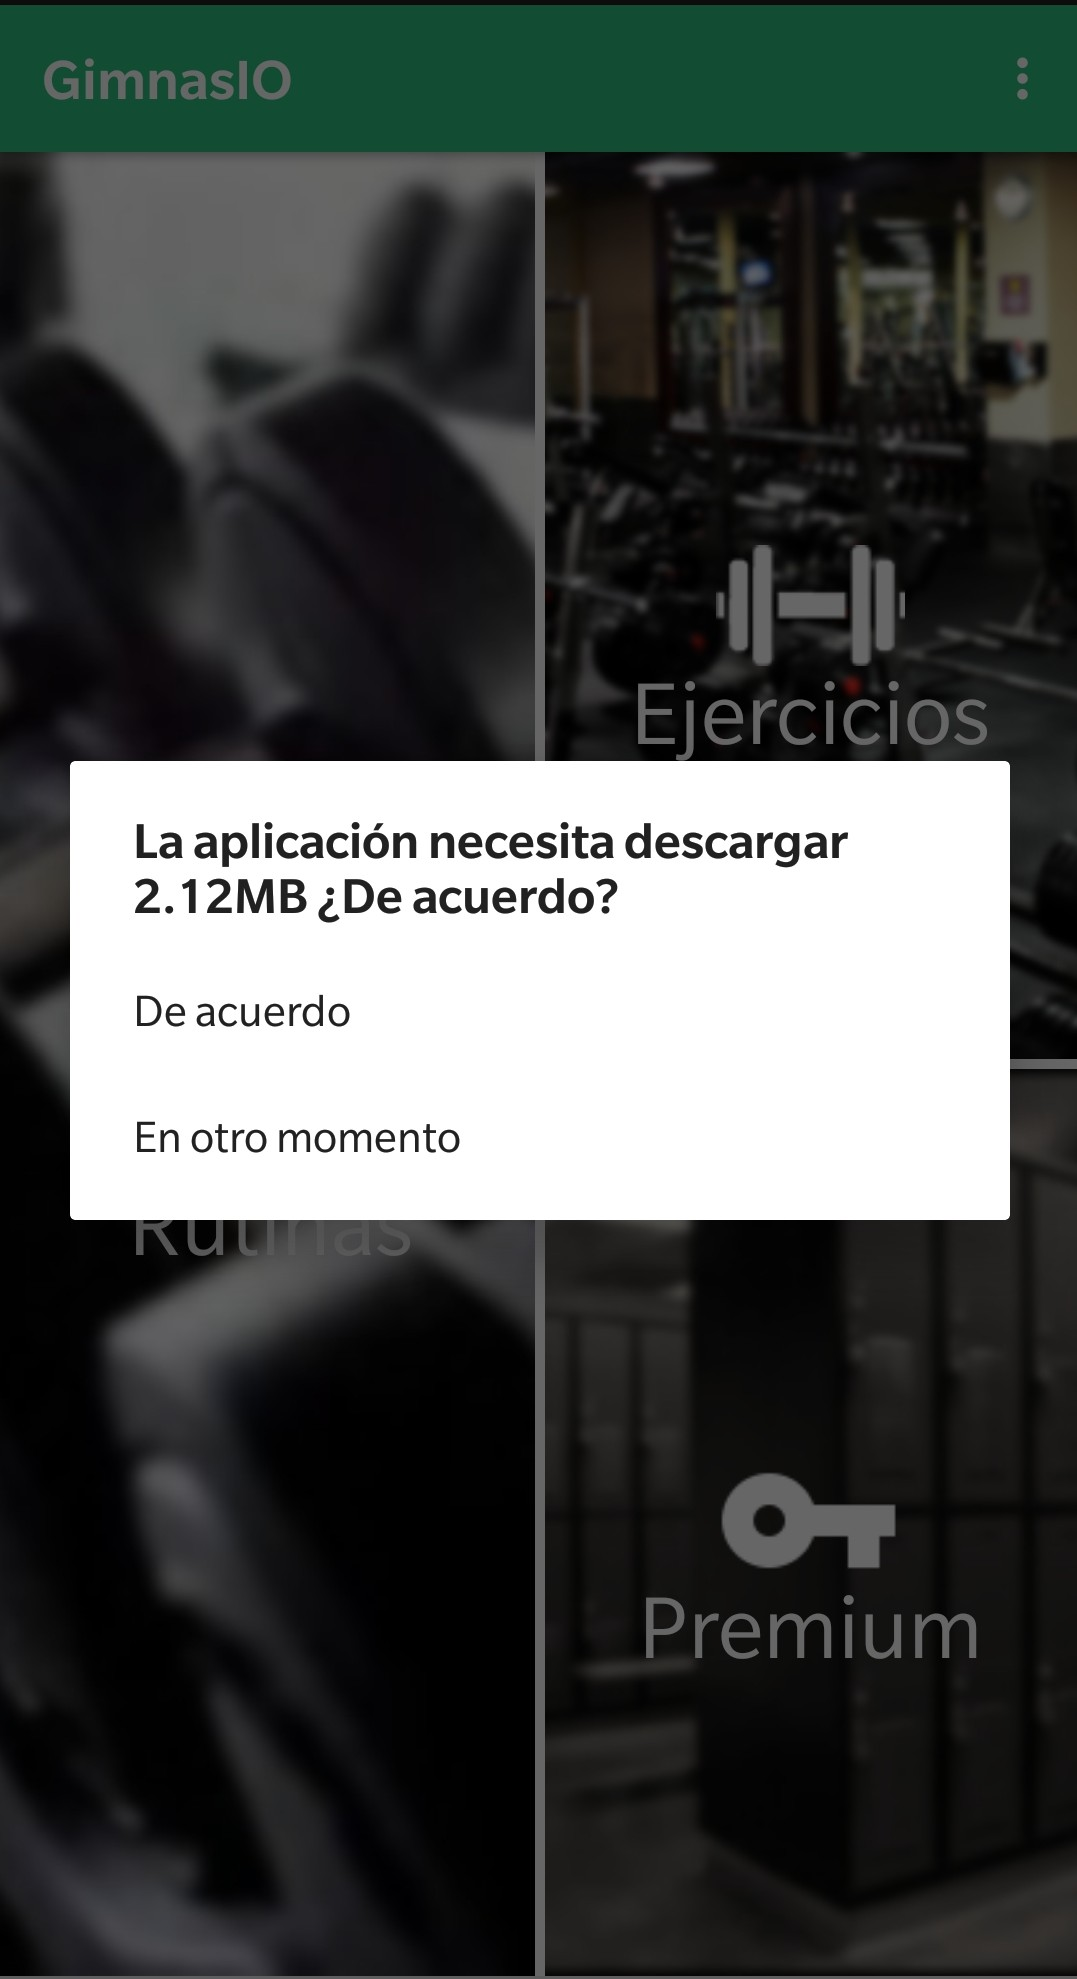
\includegraphics[width=0.3\textwidth]{graficos/manual/ConfirmacionDescarga.jpg}
	\caption{Confirmación de la descarga}
\end{figure}
Si el usuario deniega la petición de descarga, la lista de ejercicios de la aplicación se mantendrá vacía hasta que el usuario seleccione manualmente la descrga de ejercicios, por si en ese momento no dispone de conexión Wifi,o no quiera gastar datos, para que pueda posponer la descarga
\begin{figure}[H]
	\centering
	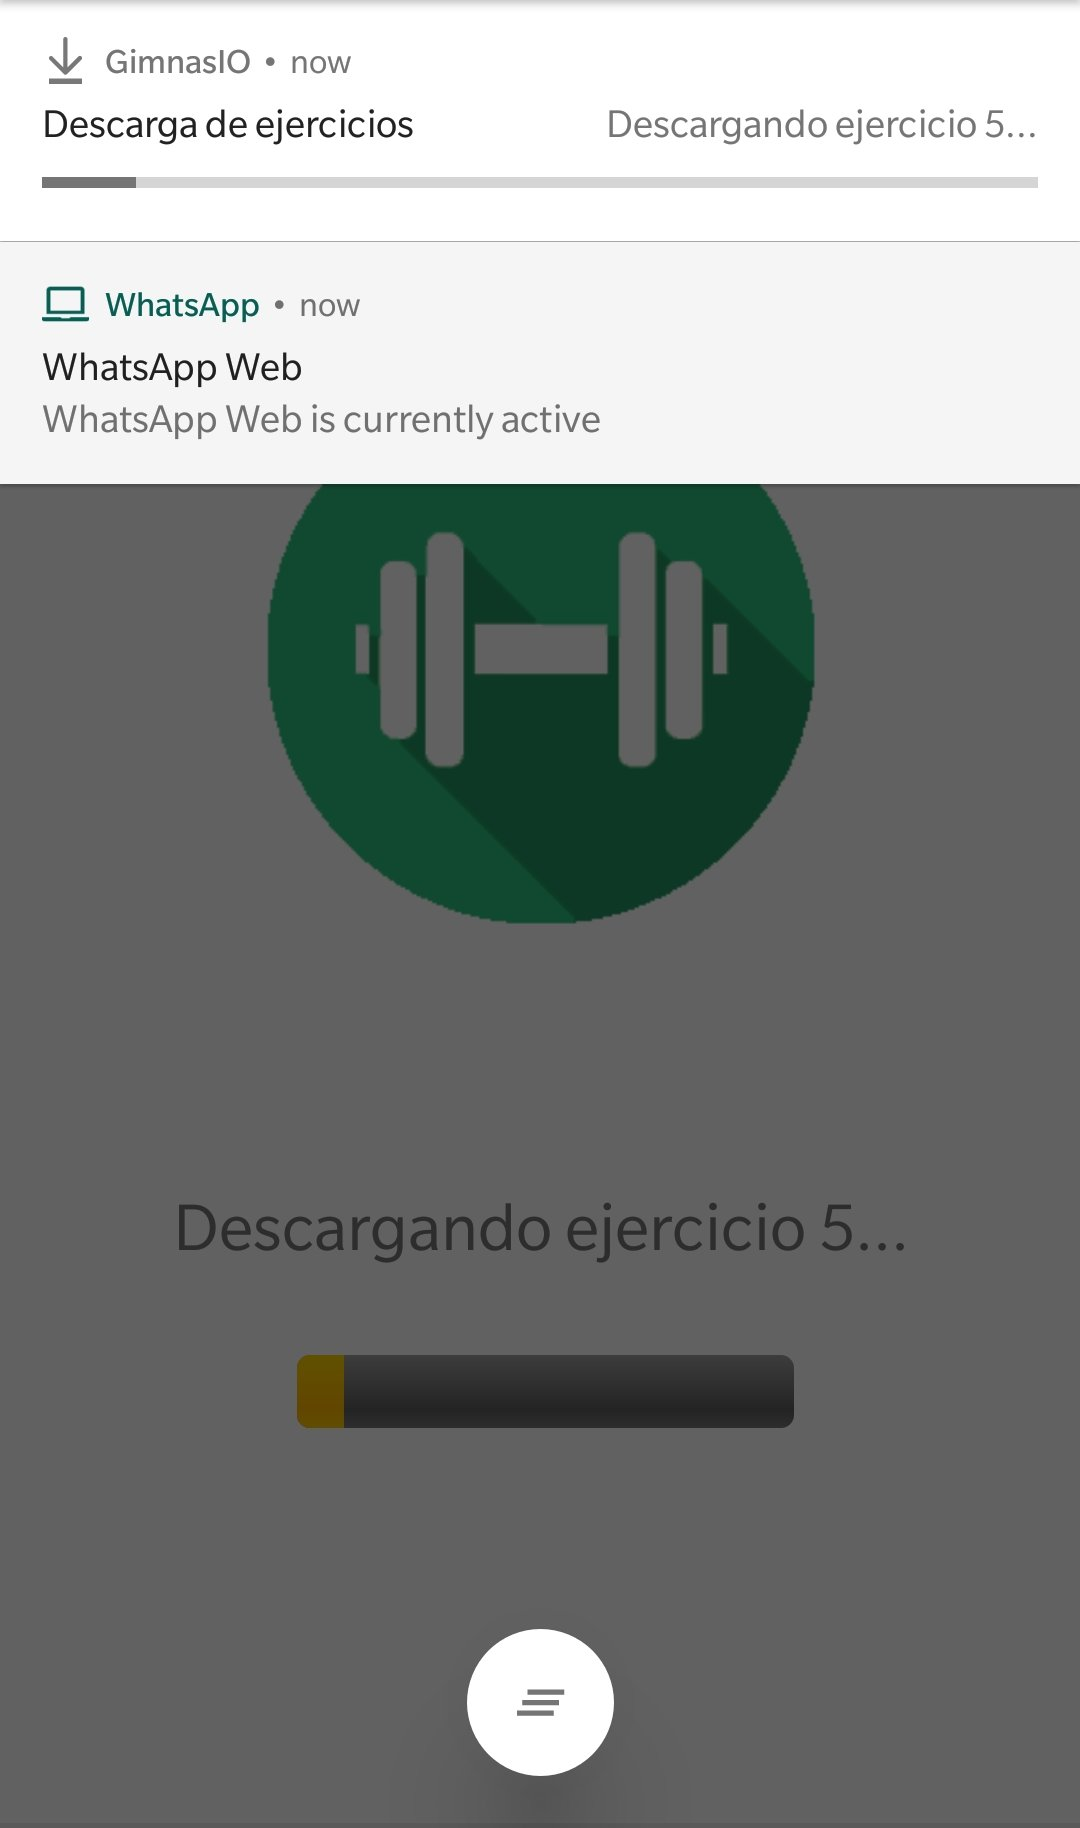
\includegraphics[width=0.3\textwidth]{graficos/manual/NotificacionDescarga.jpg}
	\caption{Notificación de la descarga}
\end{figure}
Cuando el usuario se disponga a descargar los ejercicios, la aplicación dará paso a una pantalla donde se mostrará el progreso de la descarga de los mismos. Si el usuario minimiza la aplicación, también se ha implementado una notificación en el panel superior de Android, informado del progreso de la descarga.
\begin{figure}[H]
	\centering
	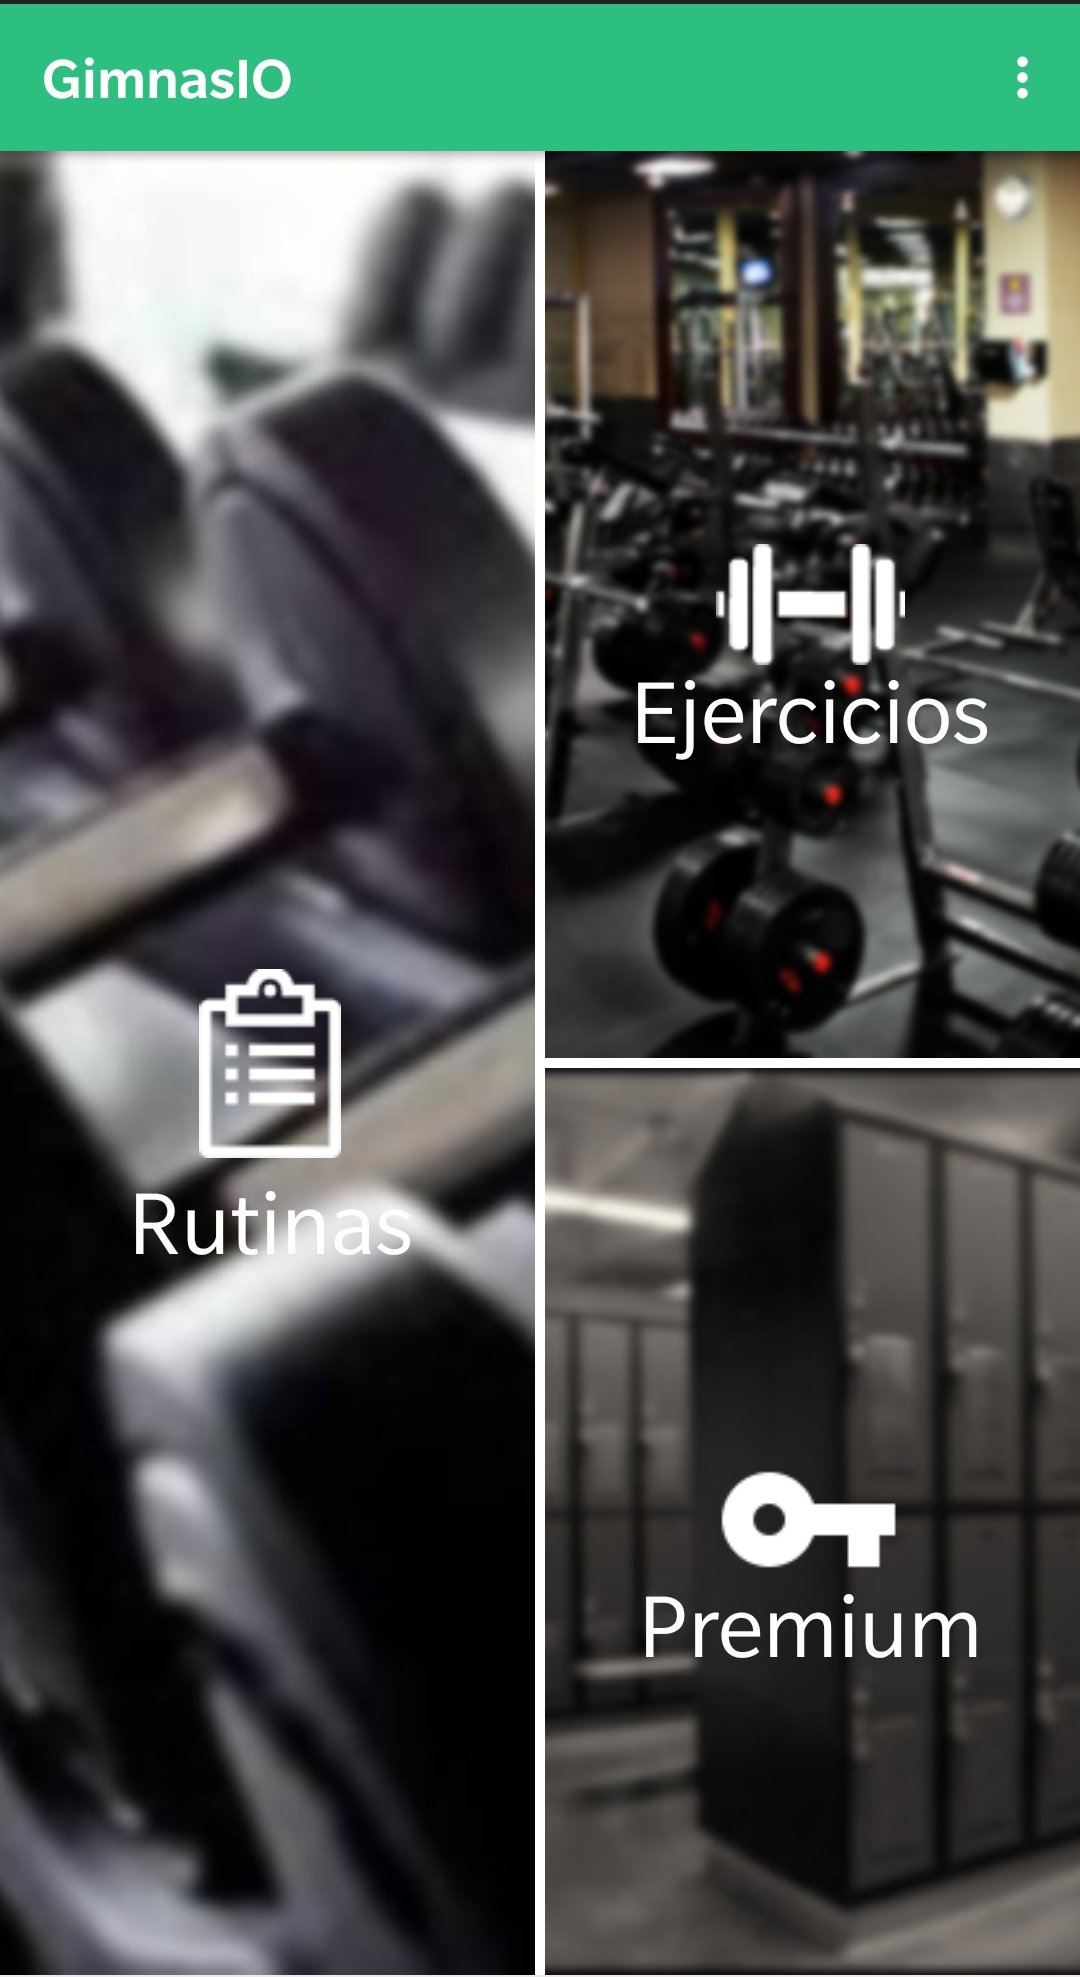
\includegraphics[width=0.3\textwidth]{graficos/manual/Menu.jpg}
	\caption{Menú principal}
\end{figure}
Una vez completada la descarga de los ejercicios, la aplicación se iniciará siempre con el menú principal, en el que hay tres botones principales, que llevarán a tres páginas distintas:
\begin{enumerate}
	\item El botón \textit{“Ejercicios”}: Se encuentra en la zona derecha, en la parte de arriba, y permite al usuario ver la lista de ejercicios disponible en la aplicación, si ha sido previamente descargada.

	\item El botón \textit{“Rutinas”}: Se encuentra ocupando toda la mitad izquierda de la pantalla, y permite al usuario interaccionar con las rutinas que se encuentran en modo local, es decir, las creadas únicamente por él. Puede añadir, eliminar, ejecutar y modificar con plena libertad.

	\item El botón \textit{“Premium”}: Se encuentra en la zona inferior de la mitad derecha, y permite al usuario, con su clave de usuario de gimnasio, o con la de coach de gimnasio, acceder a las rutinas específicas del gimnasio en el que están registrados.

\end{enumerate}
\subsubsection{Ejercicios}
\begin{figure}[H]
	\centering
	\includegraphics[width=0.3\textwidth]{graficos/manual/ListaEjercicios.jpg}
	\caption{Listado de Ejercicios}
\end{figure}
Cuando el usuario pulse el botón de ejercicios, se le redirigirá a la página mostrada arriba. La actividad se compone de una lista de ejercicios, que el usuario podrá arrastrar para ver su contenido, y un botón con una lupa que sirve para realizar la búsqueda y filtrado de ejercicios. Además, todos los ejercicios pueden ser pulsados, y los usuarios serán llevados a otra página con información más específica sobre el ejercicio seleccionado.
\begin{figure}[H]
	\centering
	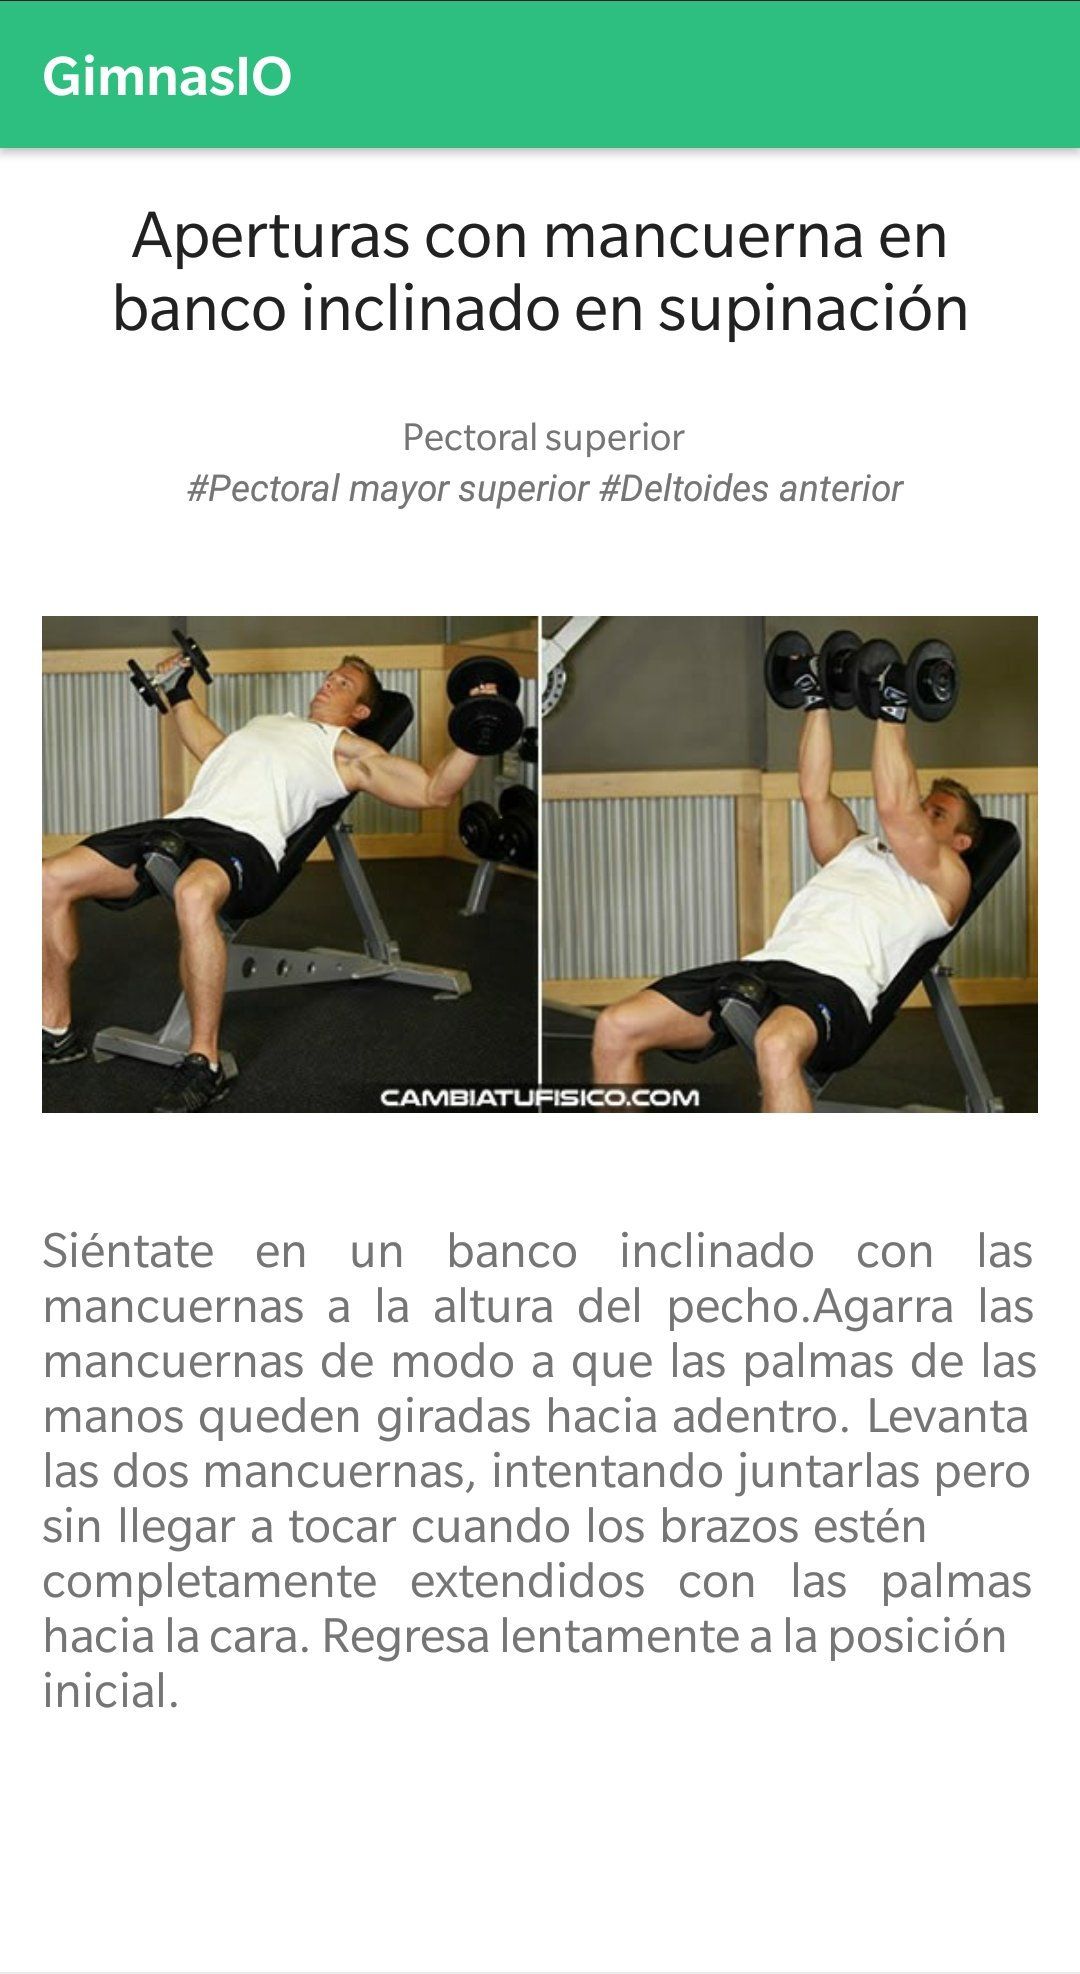
\includegraphics[width=0.3\textwidth]{graficos/manual/verEjercicio.jpg}
	\caption{Ver Ejercicio}
\end{figure}
En esta pantalla el usuario podrá observar información más detallada sobre el ejercicio, la cual se va a explicar en esta lista numerada( de arriba a abajo en la imagen):

\begin{enumerate}
	\item Nombre del ejercicio

	\item Músculo utilizado

	\item Tags del ejercicio, pequeñas referencias a músculos para que sea más fácil realizar búsquedas o para dotar de información más específica a los ejercicios.

	\item Imagen que representa el uso del ejercicio

	\item Descripción de cómo realizar el ejercicio.

\end{enumerate}
\paragraph{Búsqueda de ejercicios}

Además, también se ha incluido una opción de filtrado y búsqueda de ejercicios en la lista:
\begin{figure}[H]
	\centering
	
\includegraphics[width=0.3\textwidth]{graficos/manual/Busqueda.jpg}
	\caption{Búsqueda}
\end{figure}

Cuando el usuario presiona el botón de lupa encontrado en la zona de la barra de acción de Android, apaerece un campo en el que el usuario puede introducir la cadena de caráceteres a buscar.
\begin{figure}[H]
	\centering
	
\includegraphics[width=0.3\textwidth]{graficos/manual/SpinnerBusqueda.jpg}
	\caption{Spinner Búsqueda}
\end{figure}

Además el usuario tiene a su disposición una lista de opciones para  la búsqueda, ya que el usuario puede filtrar las rutinas según:
\begin{enumerate}
	\item Nombre

	\item Músculo

	\item Tag

\end{enumerate}
\begin{figure}[H]
	\centering
	
\includegraphics[width=0.3\textwidth]{graficos/manual/FiltradoBusqueda.jpg}
	\caption{Filtrado de Búsqueda}
\end{figure}

Una vez el usuario ha seleccionado sus preferencias de búsqueda, el programa realiza una búsqueda según dichas preferencias.
\subsubsection{Rutinas}
\begin{figure}[H]
	\centering
	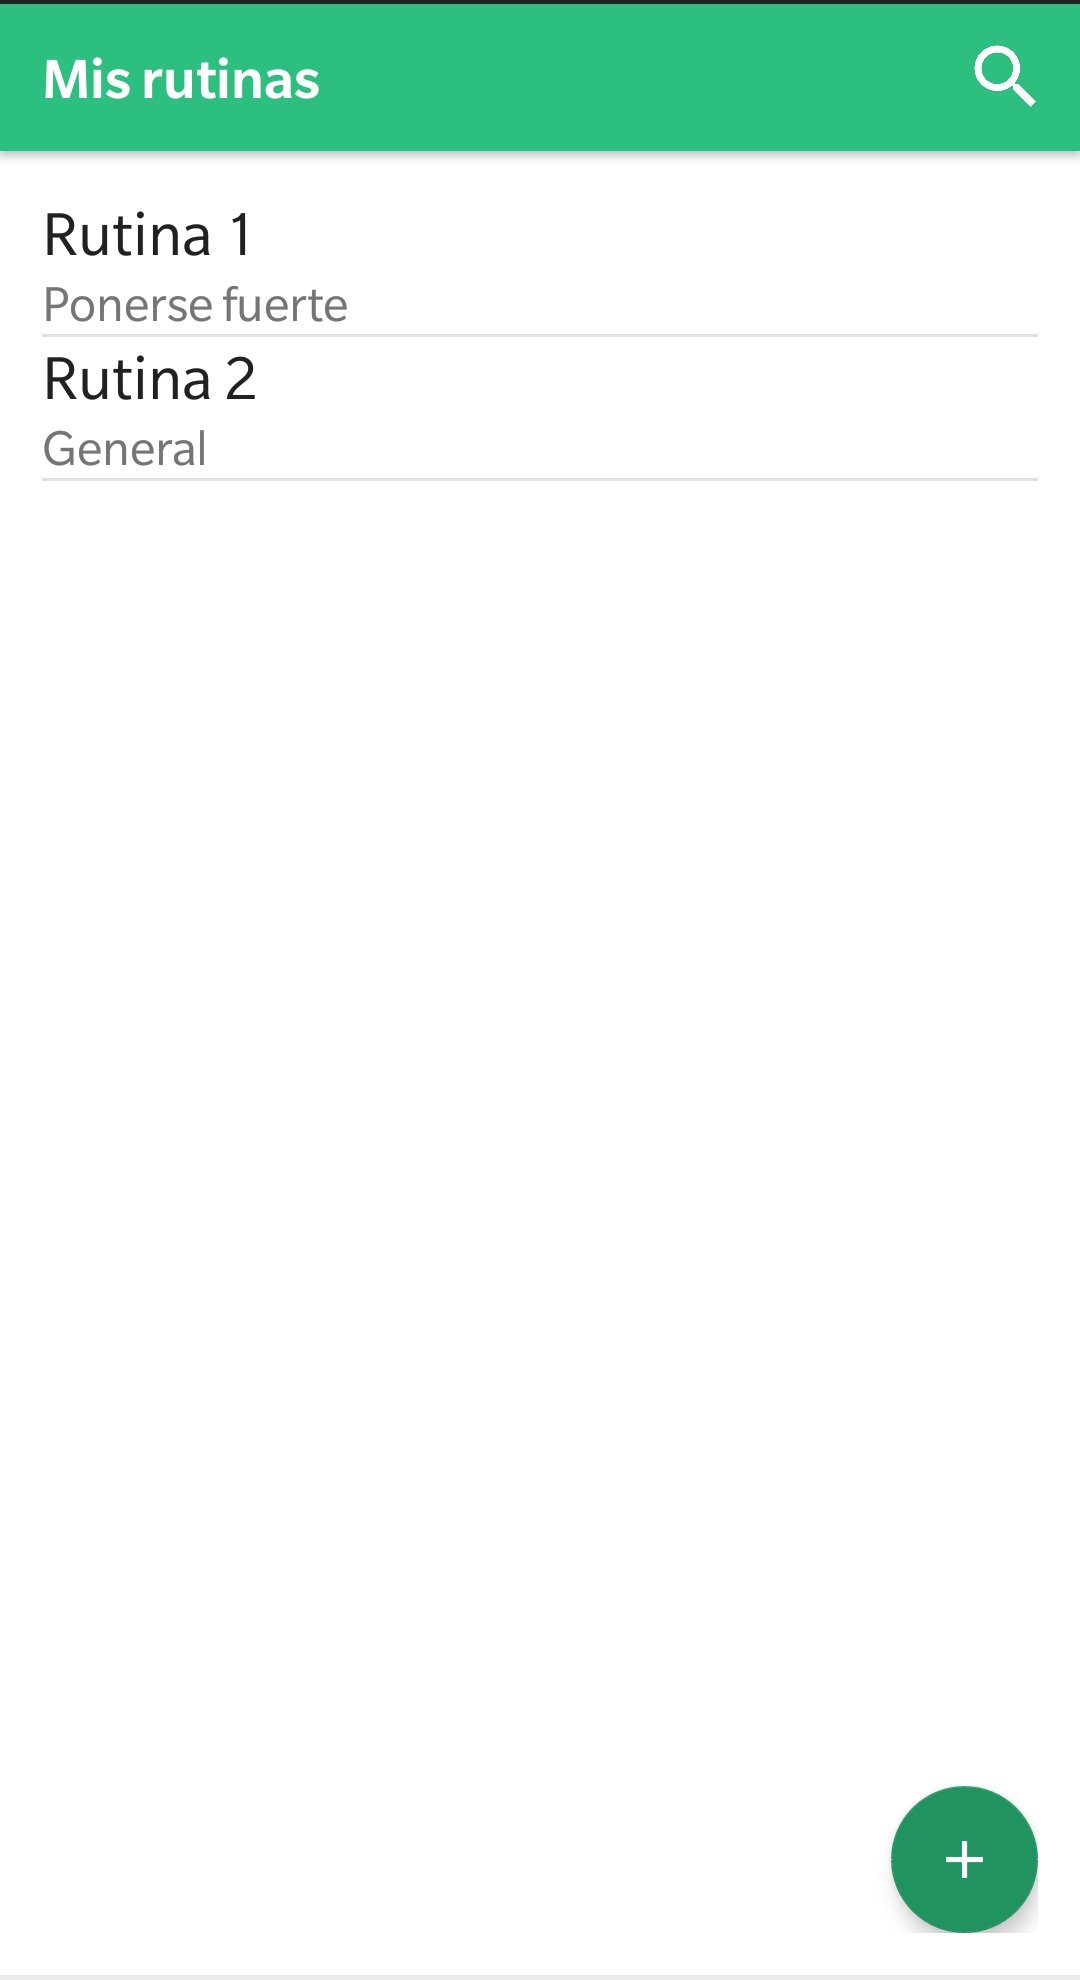
\includegraphics[width=0.3\textwidth]{graficos/manual/RutinasFreemium.jpg}
	\caption{Rutinas Freemium}
\end{figure}

Cuando el usuario selecciona la opción de “Rutinas” en el menú principal, será redirigido a una página con una lista de rutinas en local creadas por el usuario,un botón flotante que sirve para crear una rutina nueva, y una botón de búsqueda en la barra de acción de Android, que realiza un filtrado similar al de la lista de ejercicios.

\paragraph{Buscar y editar rutinas}
\begin{figure}[H]
	\centering
	\includegraphics[width=0.3\textwidth]{graficos/manual/BuscarRutinasFreemium.jpg}
	\caption{Buscar Rutinas Freemium}
\end{figure}

Los pasos a seguir para realizar la búsqueda son los mismos que en la lista de ejercicios, sólo que aquí hay dos campos por los que el usuario puede buscar:

\begin{enumerate}
	\item Nombre
	\item Objetivo de la rutina
\end{enumerate}	
Si el usuario selecciona una rutina, será direccionado a una pantalla donde puede modificar sus campos. Además, si el usuario pulsa el botón flotante de añadir, será redireccionado también a la misma página, pero con los campos para modificar en blanco, para que el usuario pueda rellenarlos.
\begin{figure}[H]
	\centering
	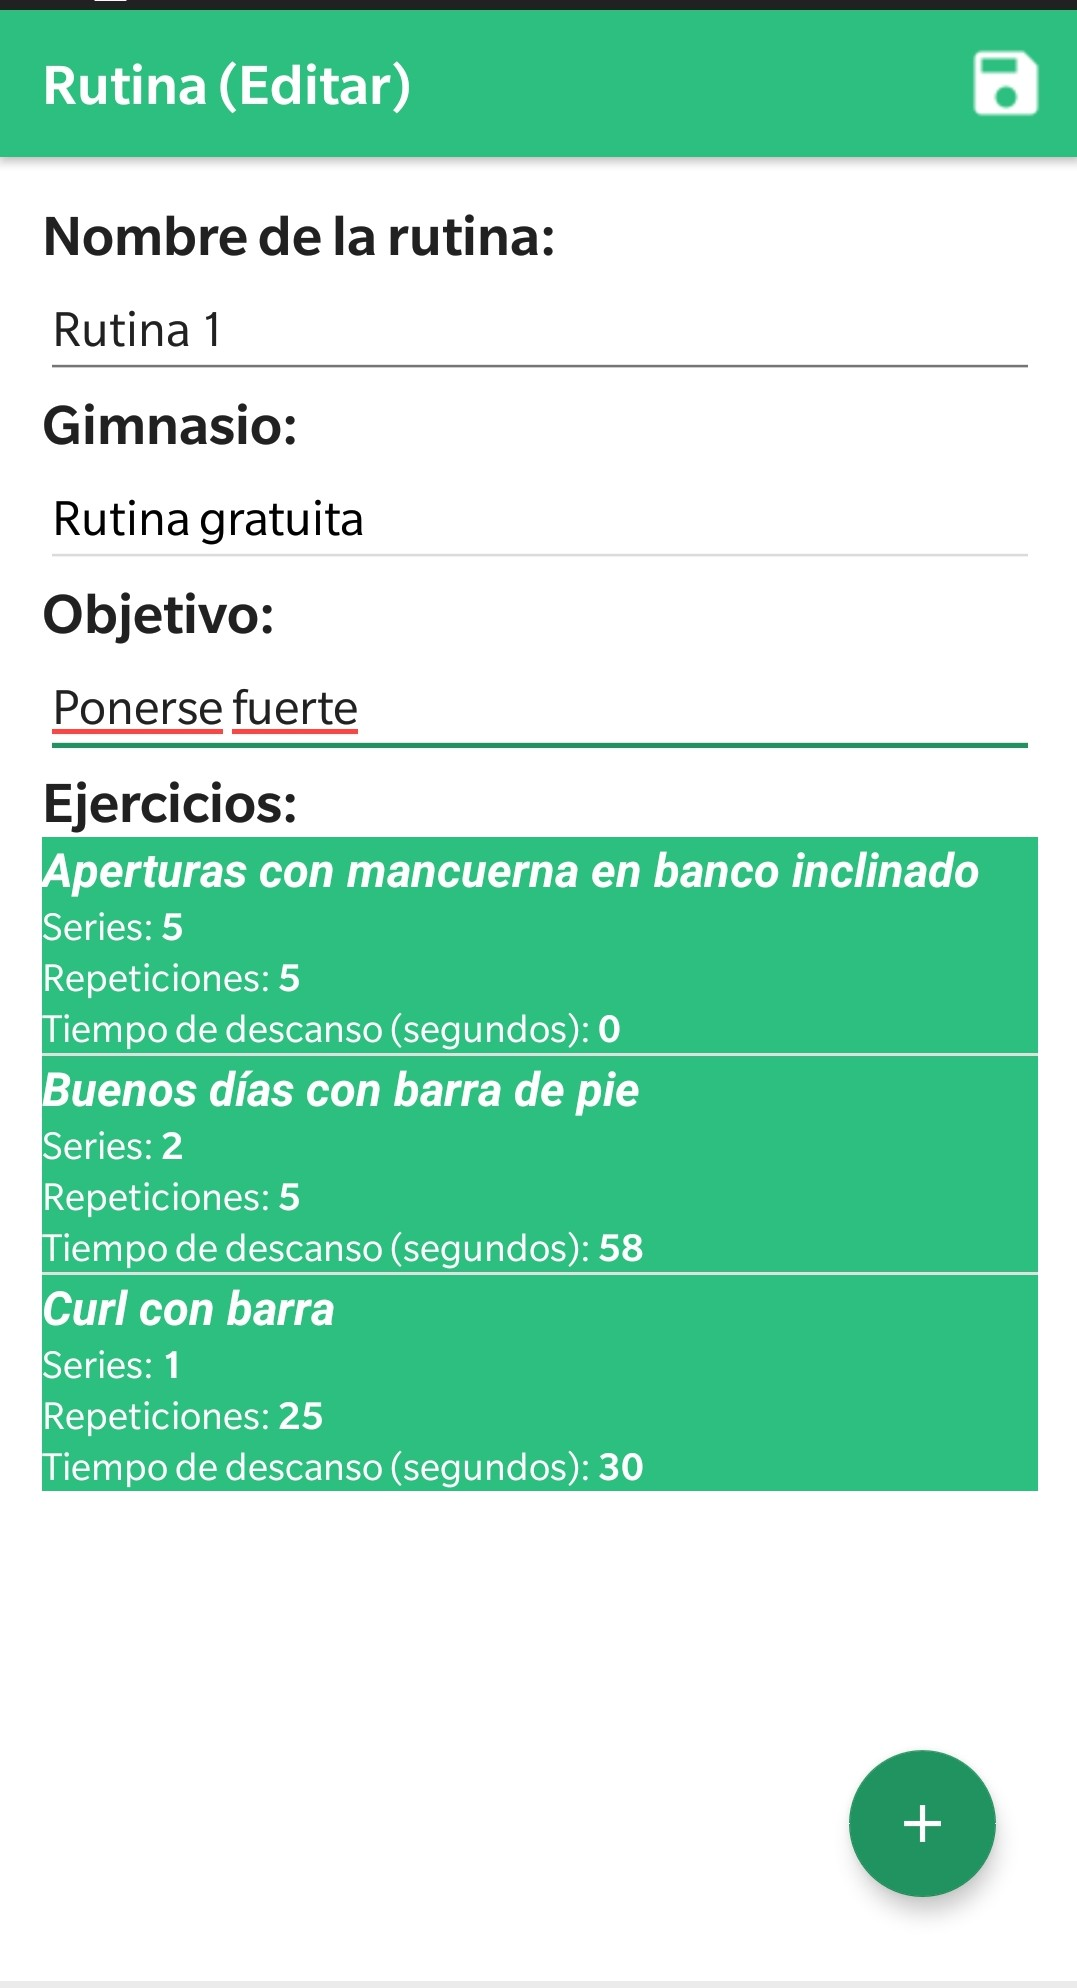
\includegraphics[width=0.3\textwidth]{graficos/manual/EditarRutina.jpg}
	\caption{Editar Rutina}
\end{figure}
En esta página podemos observar la información de la rutina:

\begin{enumerate}
	\item Nombre de la rutina

	\item Gimnasio, que indica el gimnasio que ha creado la rutina, si esta es premium.

	\item Objetivo de la rutina

	\item Lista de ejercicios

\end{enumerate}
Y un botón flotante cuya funcionalidad es añadir ejercicios a la rutina.
\\Si el usuario quiere guardar la información de la rutina, deberá pulsar el botón que se encuentra en la barra de acción, que tiene el icono de un disquete, y guardará toda modificación hecha la rutina.

\paragraph{Añadir ejercicios a rutina}
\begin{figure}[H]
	\centering
	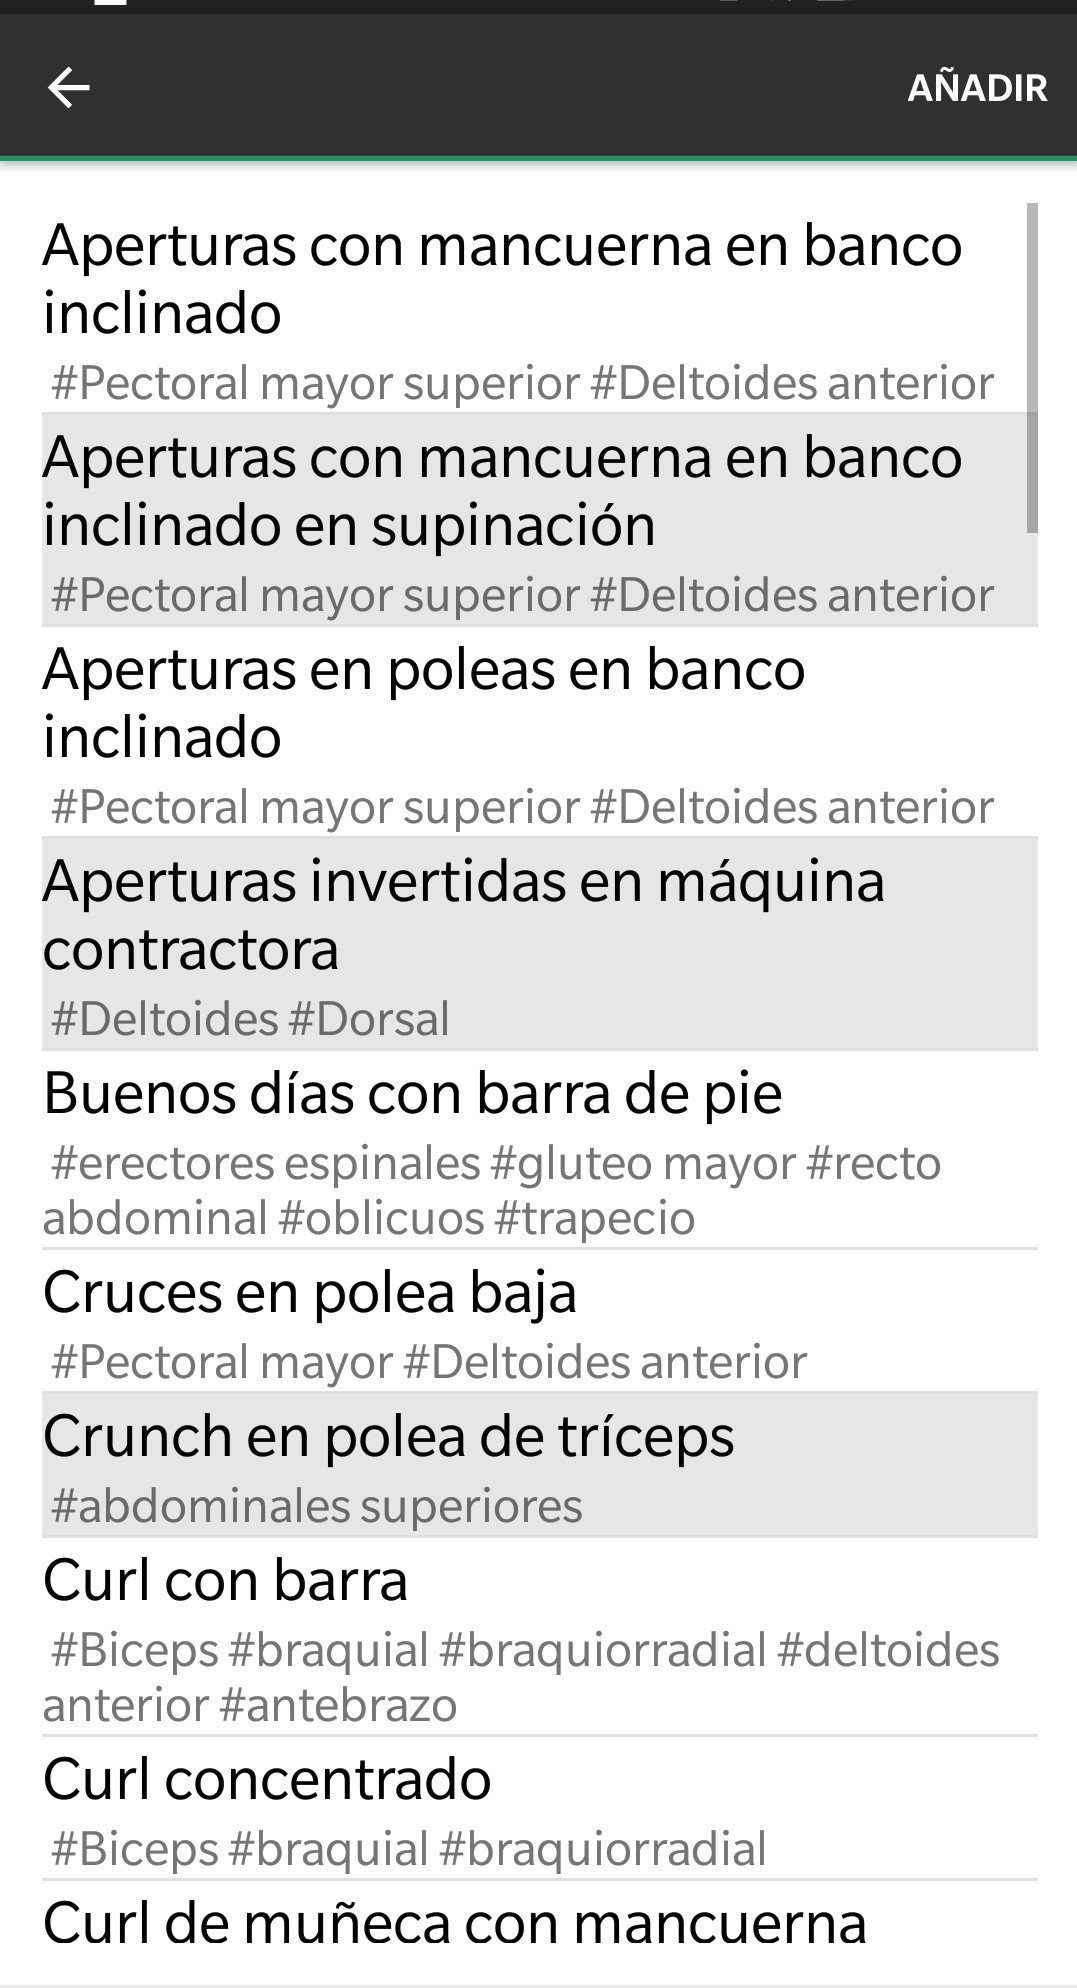
\includegraphics[width=0.3\textwidth]{graficos/manual/AnadirEjercicioLista.jpg}
	\caption{Añadir ejercicio a la lista}
\end{figure}
Si el usuario pulsa el botón de añadir ejercicios, será redirigido a la lista de ejercicios disponibles, en la que el usuario podrá seleccionar uno o más ejercicios y añadirlos a la rutina. Los ejercicios seleccionados cambiarán a un color más oscuro para indicar al usuario que están seleccionados.
\begin{figure}[H]
	\centering
	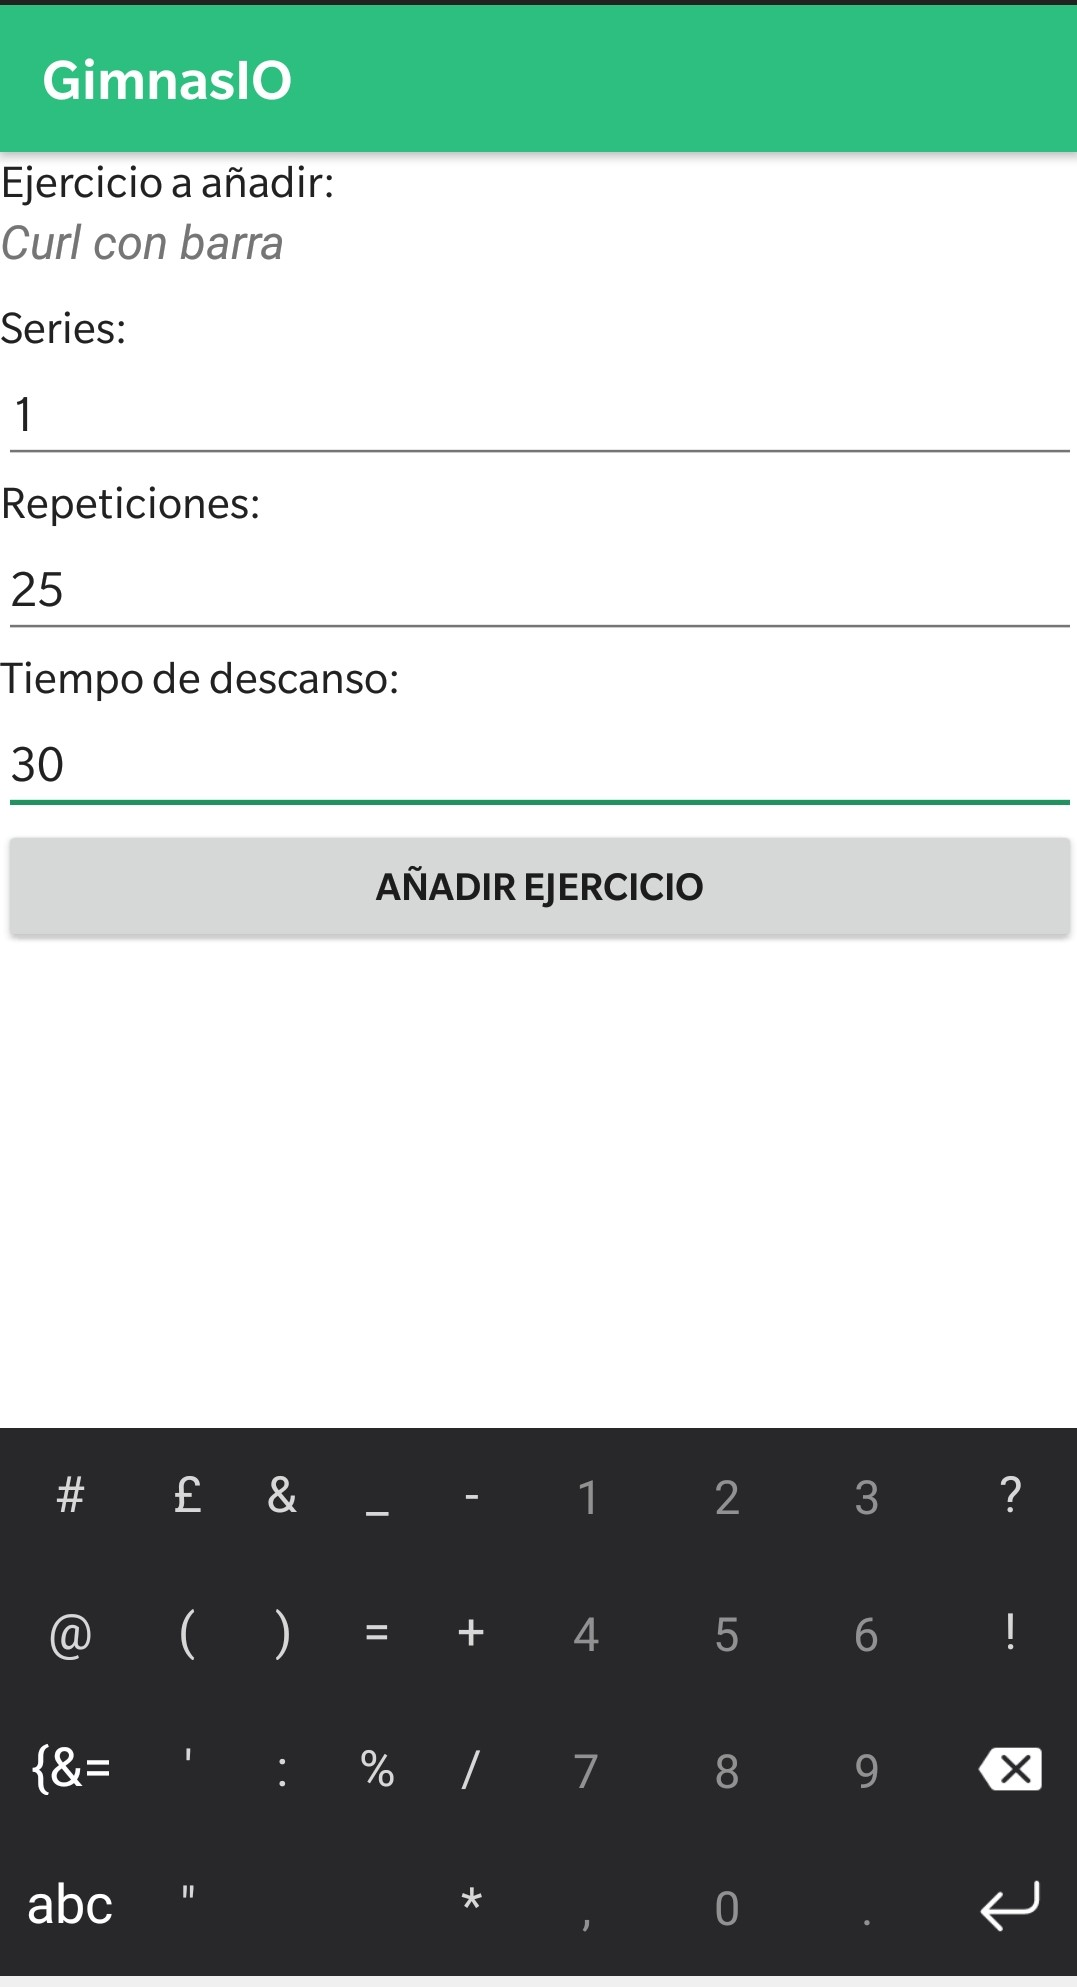
\includegraphics[width=0.3\textwidth]{graficos/manual/AnadirEjercicio.jpg}
	\caption{Añadir ejercicio}
\end{figure}
Cuando el usuario seleccione los ejercicios, también tiene que seleccionar otros atributos del mismo:
\begin{enumerate}
	\item Número de series del ejercicio

	\item Número de repeticiones de cada serie

	\item Tiempo de descanso entre series

\end{enumerate}
\begin{figure}[H]
	\centering
	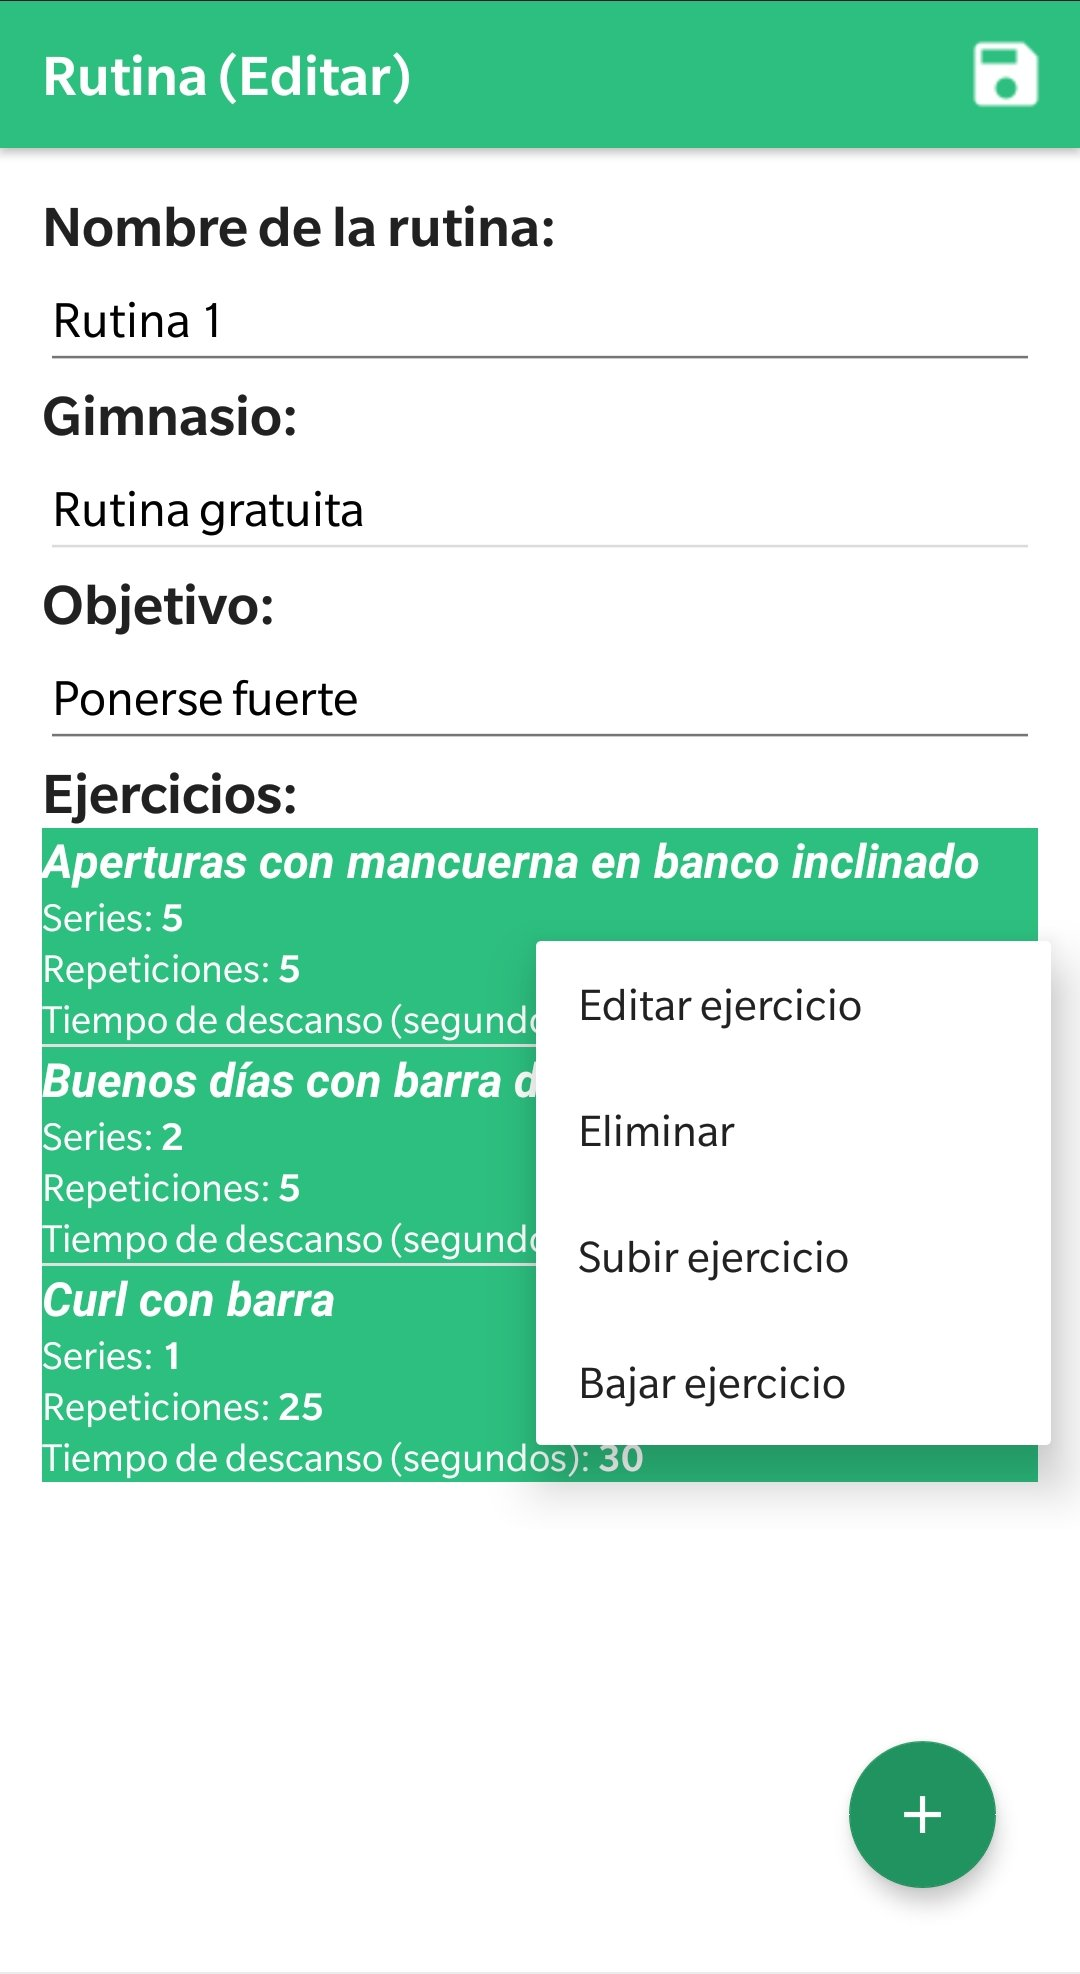
\includegraphics[width=0.3\textwidth]{graficos/manual/MenuEjercicioEnRutina.jpg}
	\caption{MenuEjercicioEnRutina}
\end{figure}
Al añadir los ejercicios, el usuario también tiene la posibilidad de modificar esta lista según sus necesidades, ya que al seleccionar un ejercicio de la lista se le abrirá un menú con estas opciones:
\begin{enumerate}
	\item Editar ejercicio, en la que el usuario podrá cambiar cualquiera de los tres campos( series,repeticiones, tiempo de descanso) del ejercicio seleccionado.
	\item Eliminar ejercicio de la lista de ejercicios de la rutina
	\item Subir ejercicio una posición, para que se ejecute una posición antes.

	\item Bajar ejercicio una posición, para que se ejecute una posición después.
\end{enumerate}
\paragraph{Ejecutar rutina}
Cuando el usuario ha seleccionado una rutina, también puede ejecutar la rutina, que consiste en que la aplicación enseñará los ejercicios a realizar, además de información sobre el tiempo de descanso, y el tiempo total invertido en la rutina.
\begin{figure}[H]
	\centering
	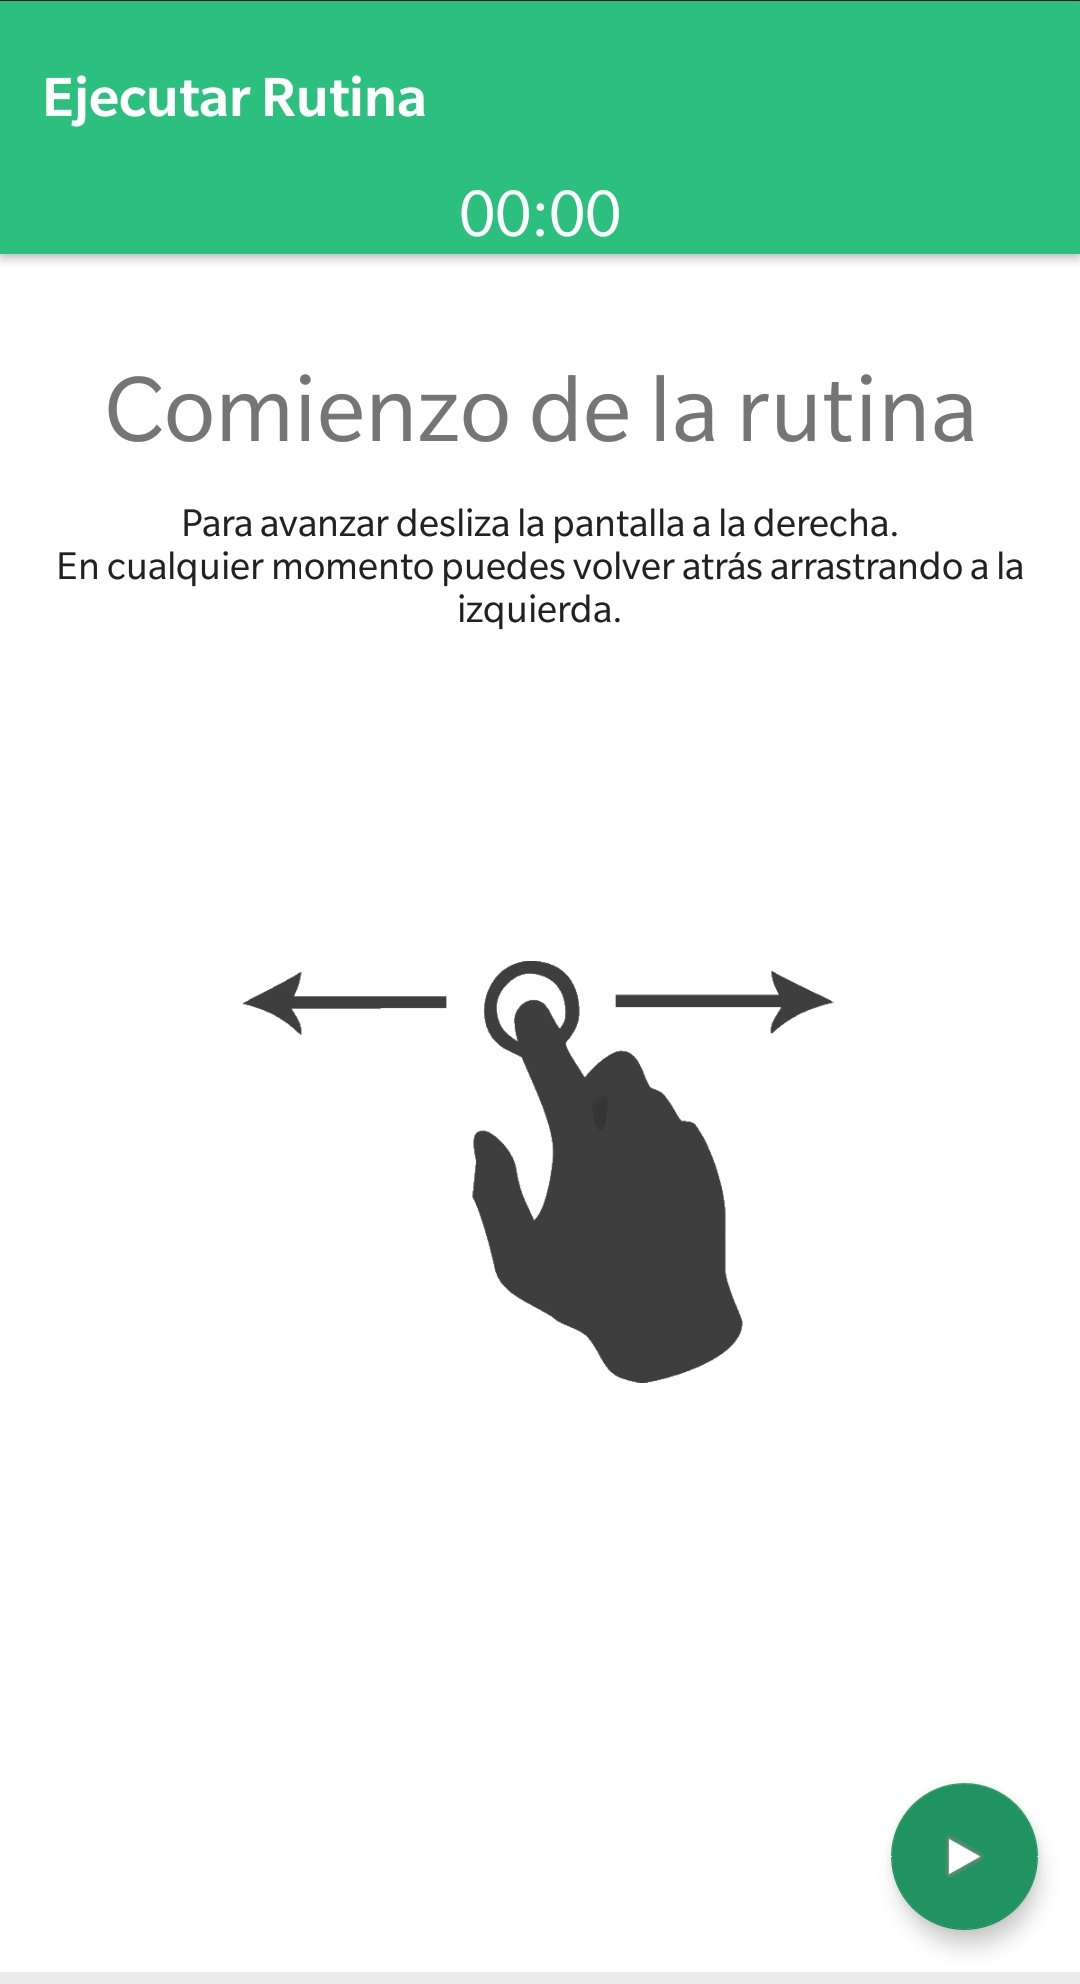
\includegraphics[width=0.3\textwidth]{graficos/manual/EmpezarRutina.jpg}
	\caption{Empezar una rutina}
\end{figure}
En la pantalla de inicio de la rutina, se muestra información sobre cómo avanzar de ejercicio, que se hace arrastrando la pantalla hacia la derecha, y se incluye un gif que sirve de ayuda.
\begin{figure}[H]
	\centering
	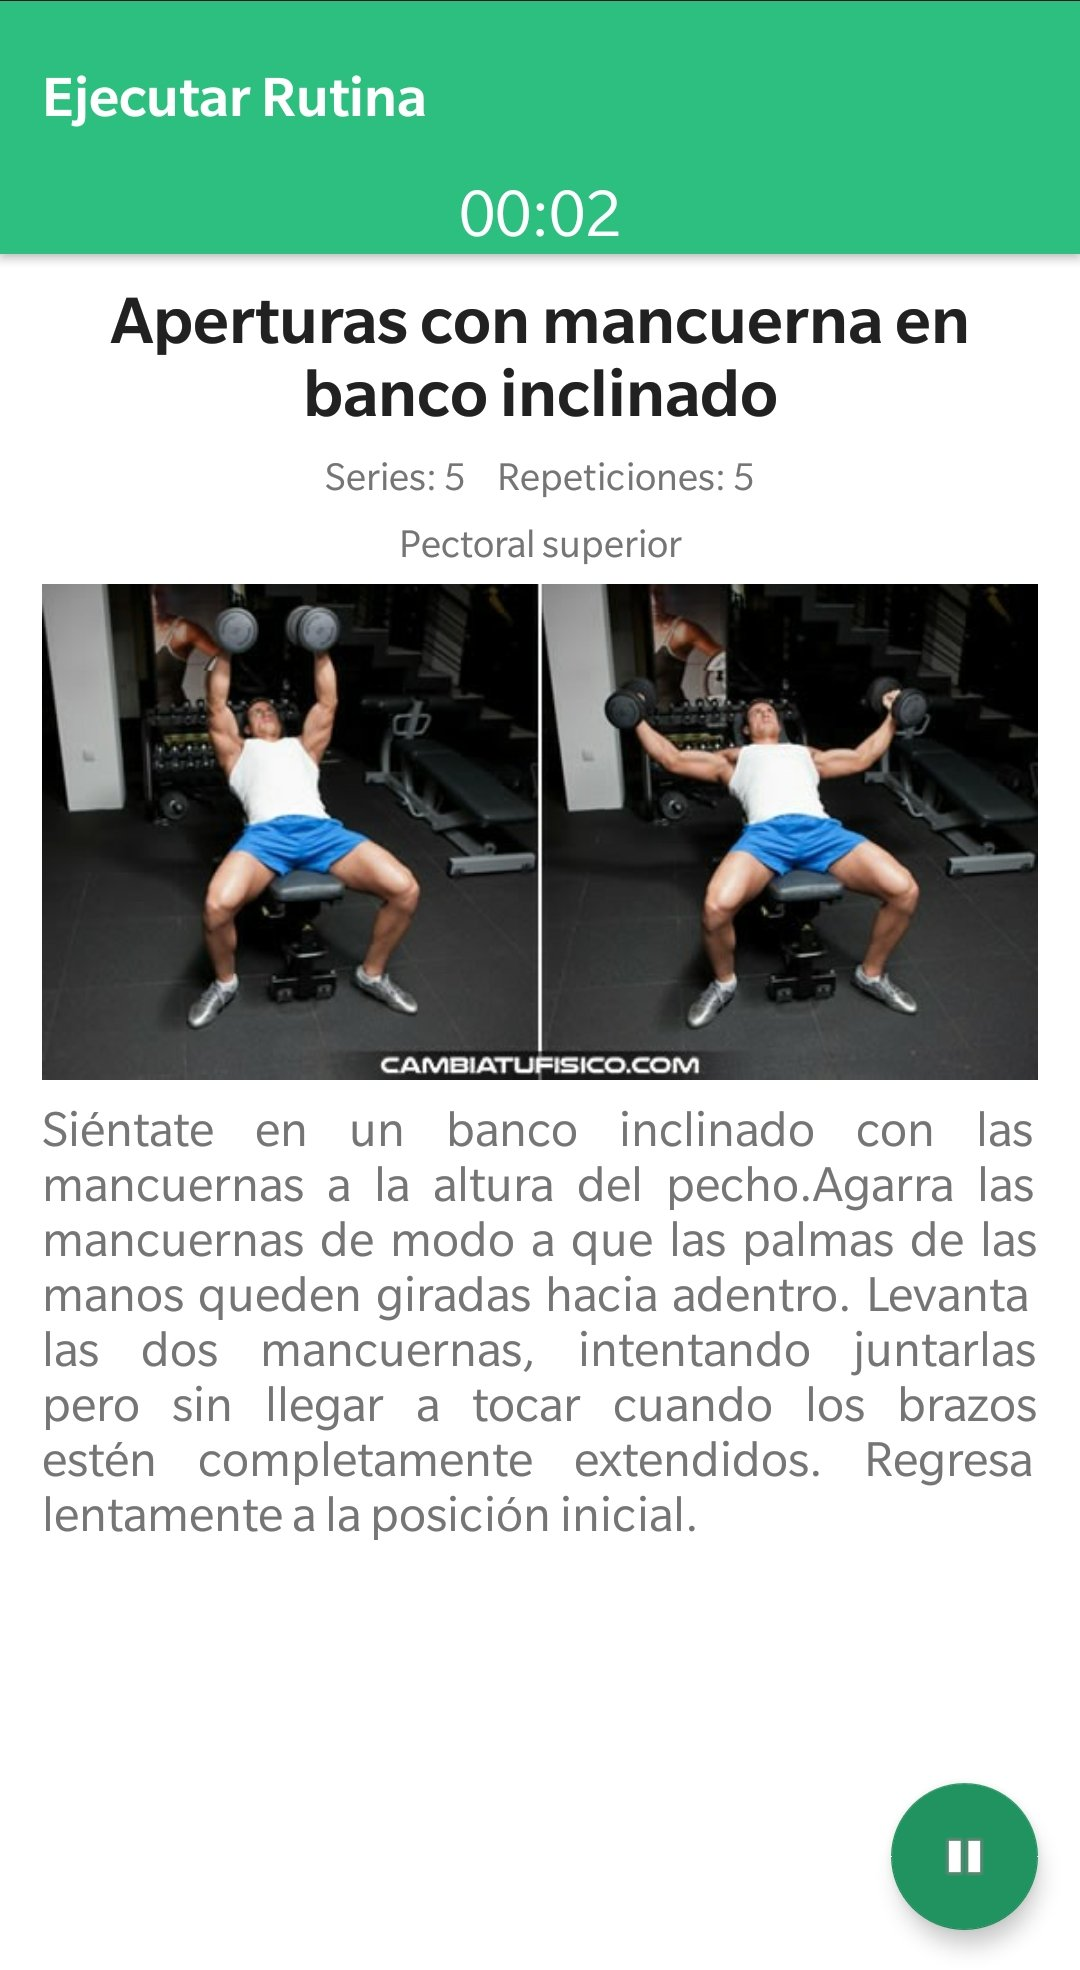
\includegraphics[width=0.3\textwidth]{graficos/manual/EjercicioEnEmpezarRutina.jpg}
	\caption{Ejercicio en ejecución de rutina}
\end{figure}

En esta pantalla se muestra el ejercicio al ejecutar la rutina. Incluye en la zona superior el tiempo total invertido en la rutina, y un botón de pausa por si se quiere empezar/parar el contador. Además, incluye la información perteneciente al ejercicio, series, repeticiones y músculo usado.

\begin{figure}[H]
	\centering
	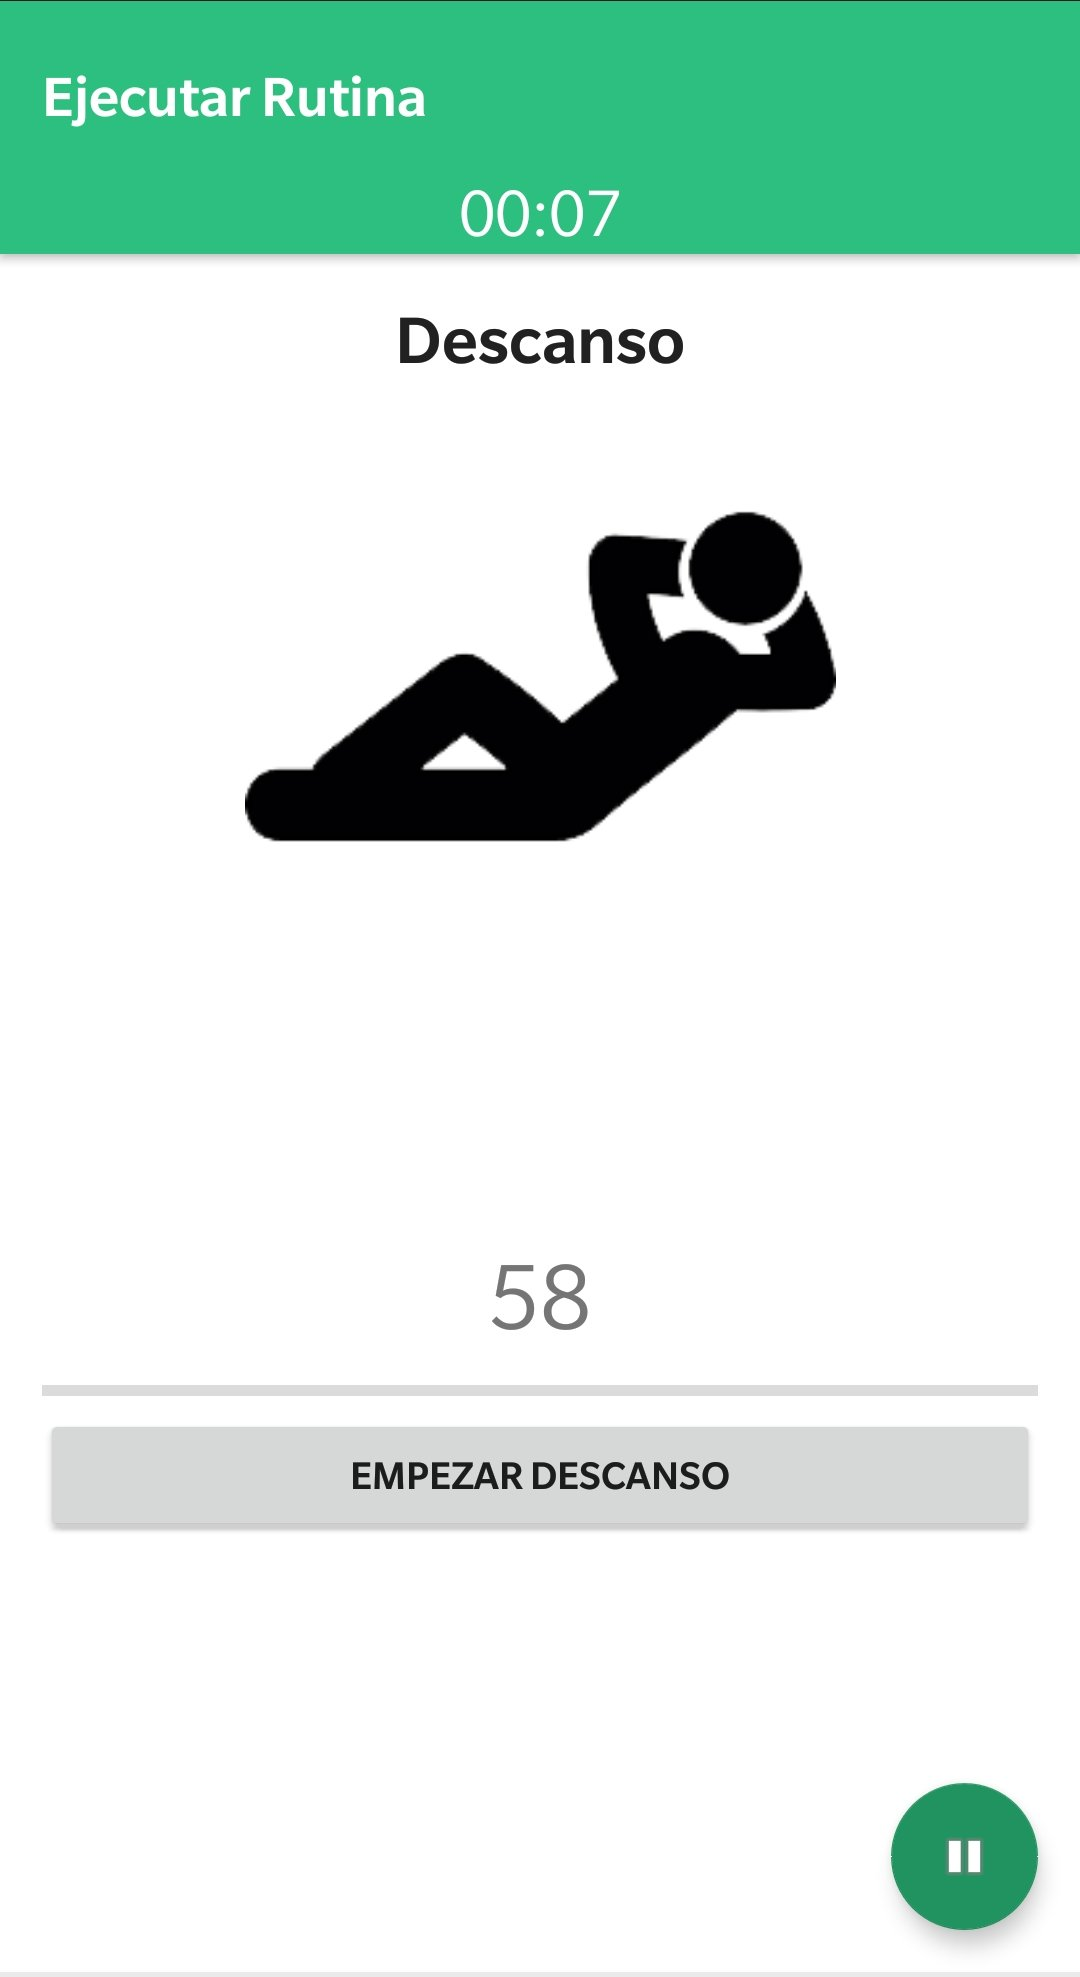
\includegraphics[width=0.3\textwidth]{graficos/manual/PantallaDescanso.jpg}
	\caption{Pantalla de descanso}
\end{figure}
En esta pantalla se calcula el tiempo de descanso de cada ejercicio. Una vez terminado el tiempo, el usuario puede continuar al siguiente ejercicio, y así hasta el final de la lista de ejercicios de la rutina.

\begin{figure}[H]
	\centering
	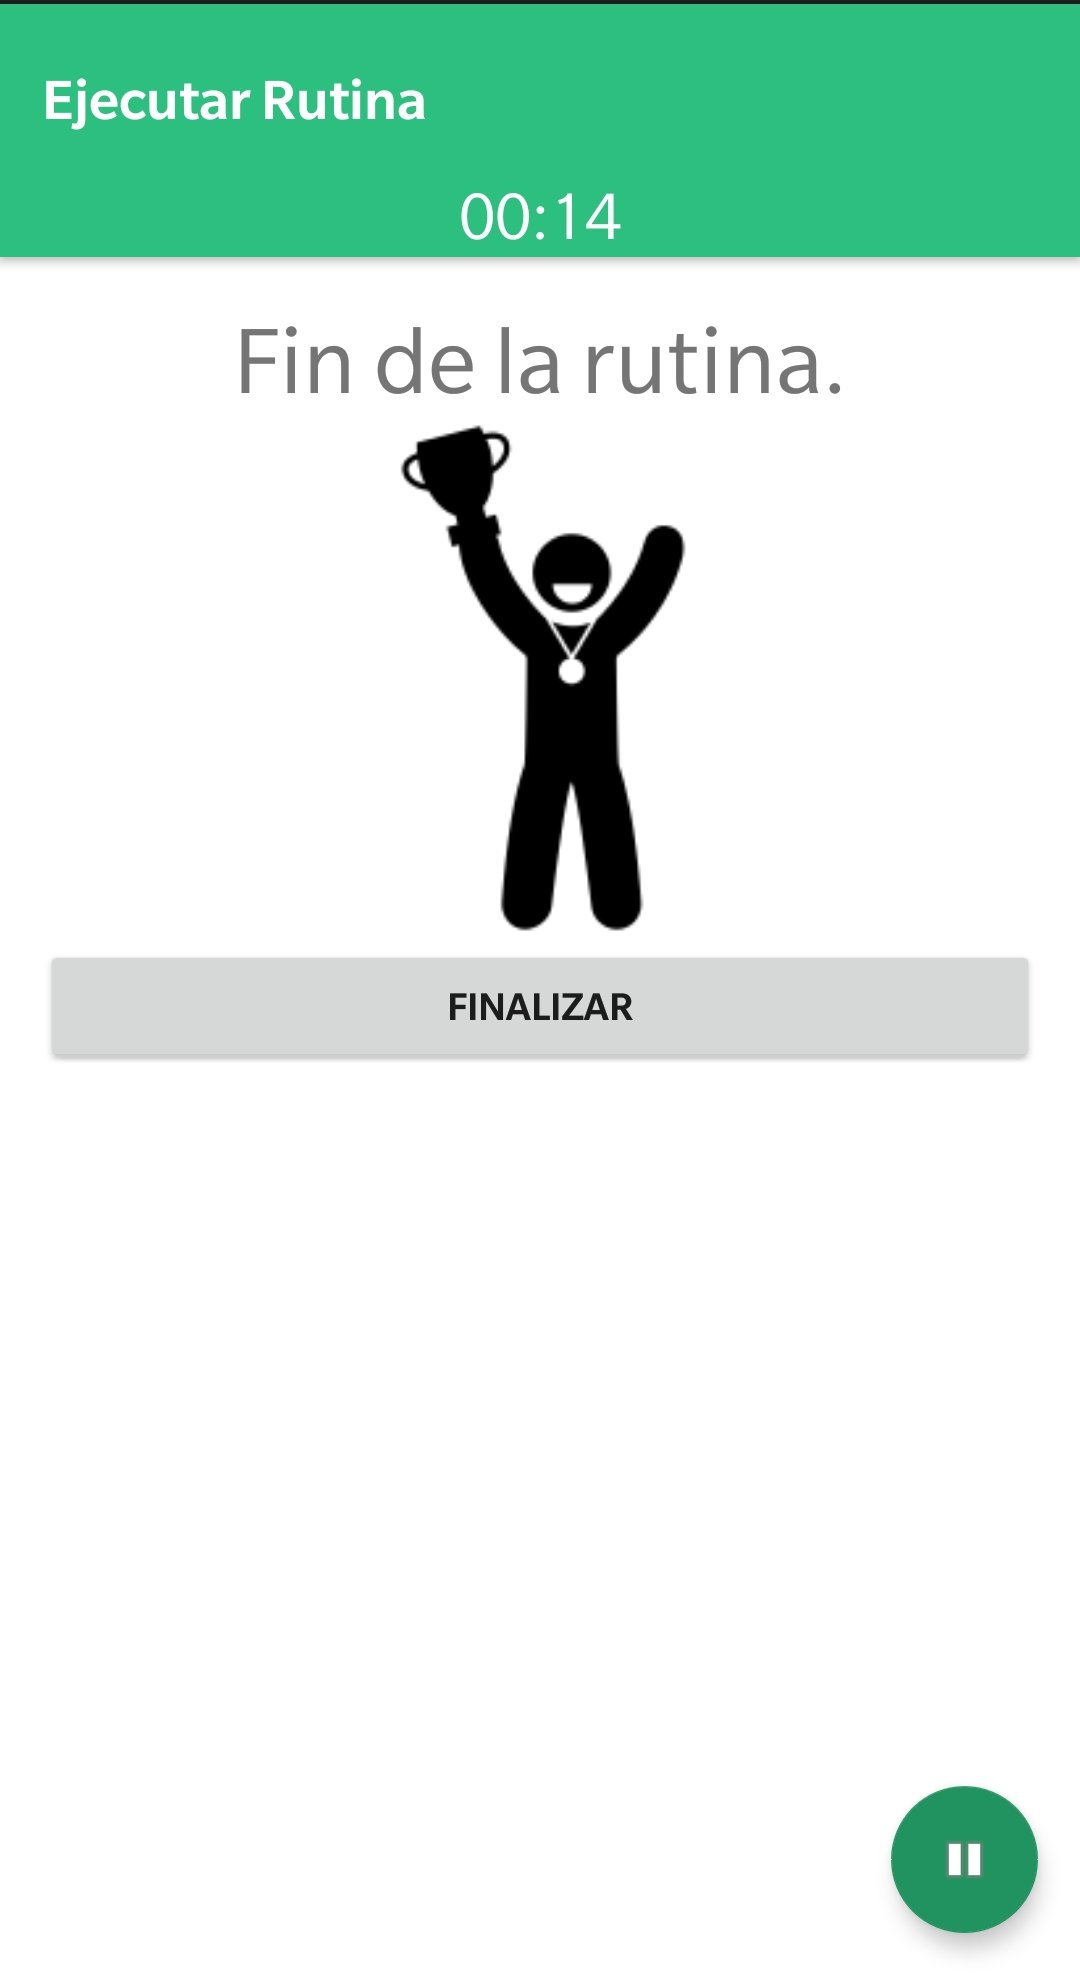
\includegraphics[width=0.3\textwidth]{graficos/manual/FinRutina.jpg}
	\caption{Final de la rutina}
\end{figure}
Al finalizar la rutina, se mostrará la pantalla de final de rutina, y si el usuario pulsa el botón “Finalizar”, se le devuelve a la pantalla de edición de rutina.

\paragraph{Borrar rutinas}
\begin{figure}[H]
	\centering
	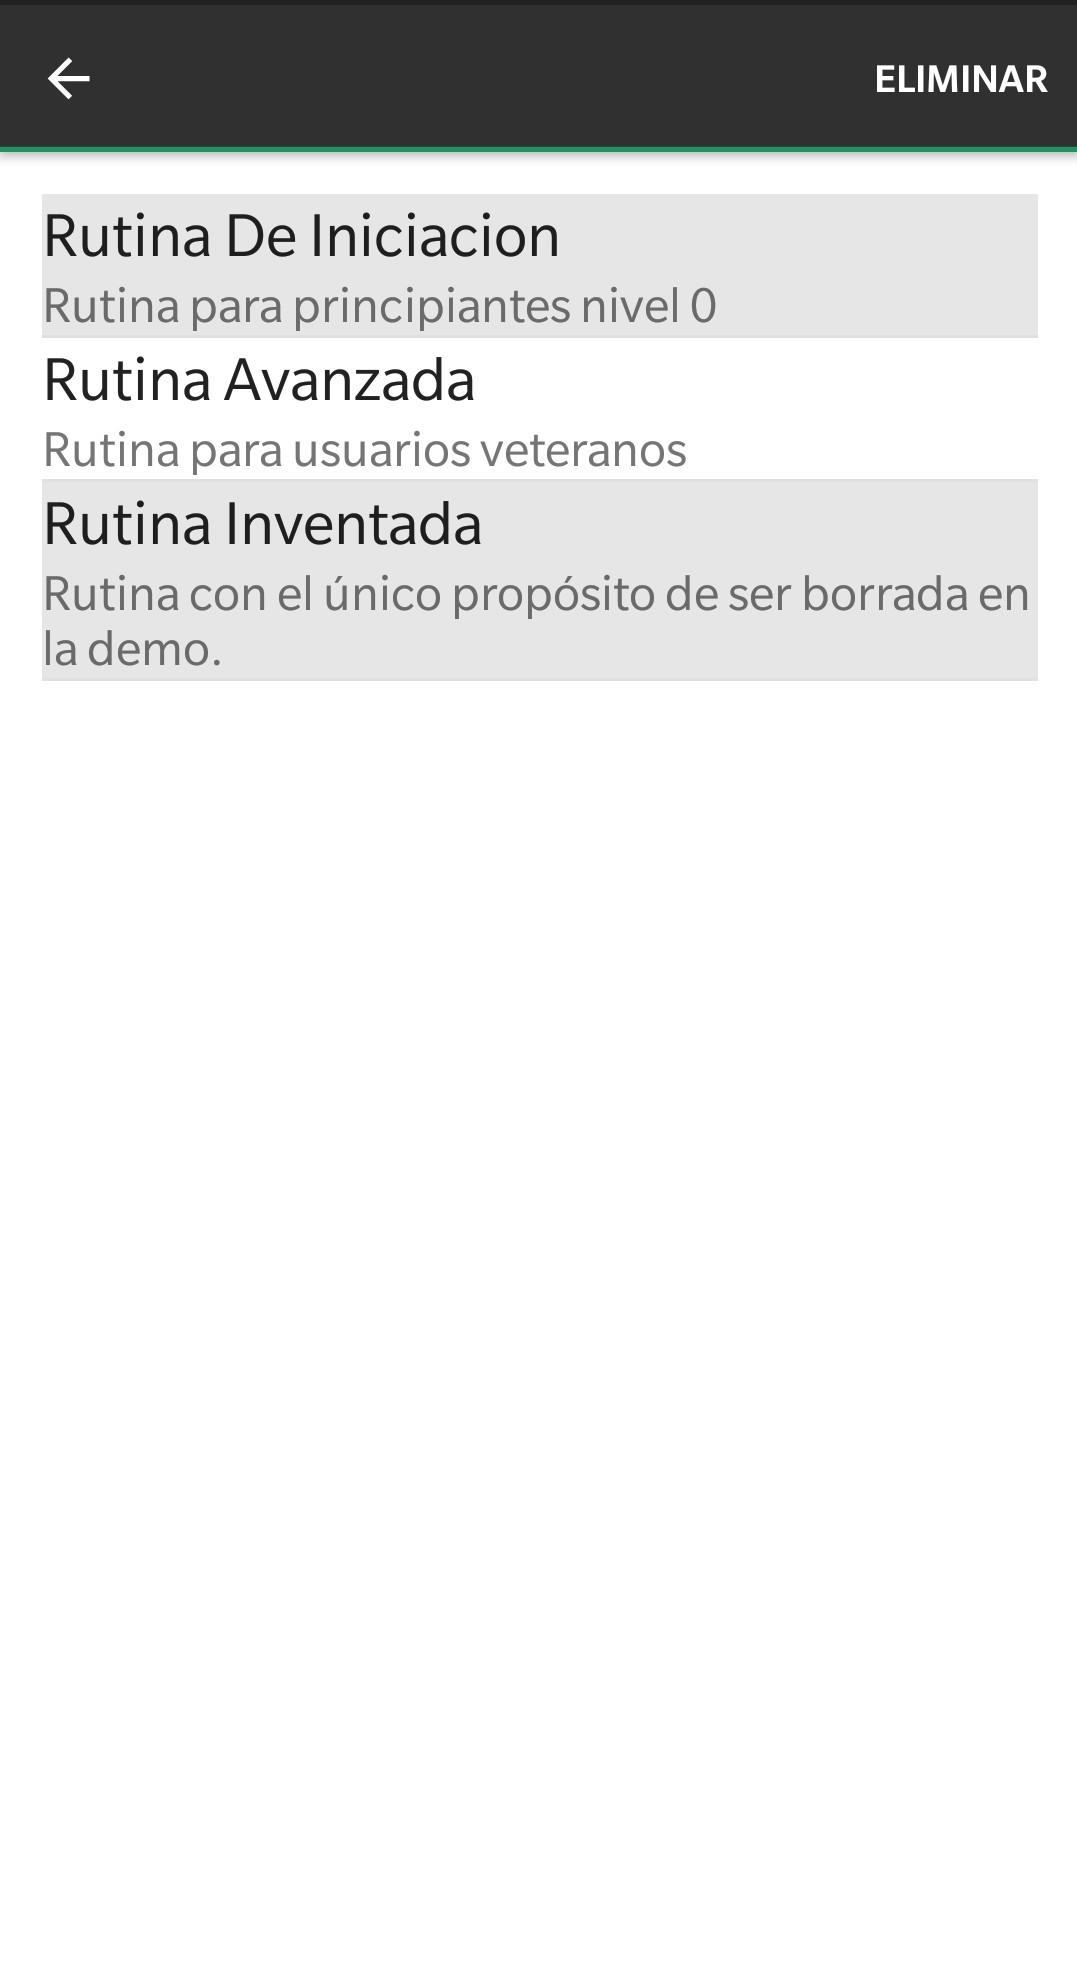
\includegraphics[width=0.3\textwidth]{graficos/manual/BorrarRutinasFreemium.jpg}
	\caption{Borrado de rutinas freemium}
\end{figure}
Para borrar las rutinas, el usuario debe mantener pulsado las rutinas que quiere eliminar, las cuales se marcarán poniéndose en un tono más oscuro, y cuando haya seleccionado todas, pulsar el botón de “Eliminar” que se encuentra en la barra de acción.

\subsubsection{Registro en servicio premium}

Para poder tener acceso a un sistema premium personalizado para el gimnasio, primero, algún representante del gimnasio debe  registrarse en la dirección \url{http://54.171.225.70:32001/registrate}. 

\begin{figure}[H]
	\centering
	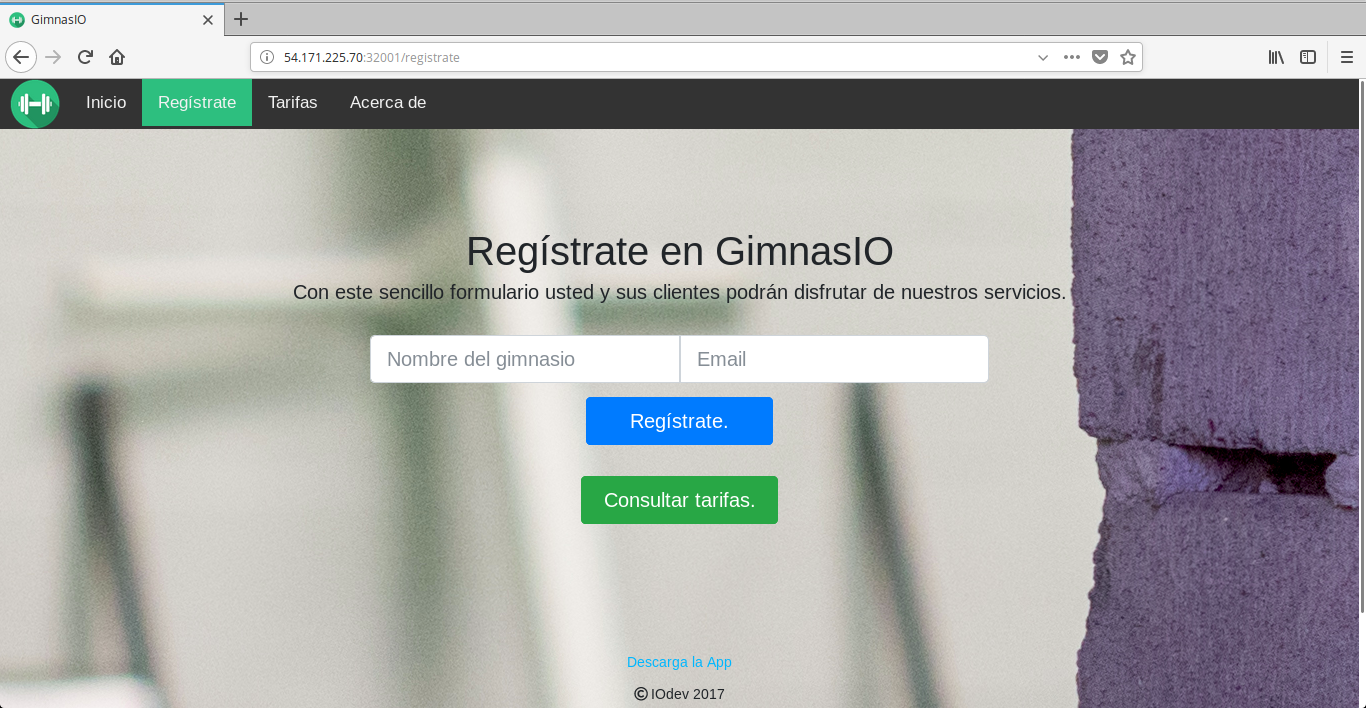
\includegraphics[width=0.9\textwidth]{graficos/manual/RegistroWeb.png}
	\caption{Registro Web}
\end{figure}
Una vez introducido el nombre del gimnasio y un correo, el usuario debe hacer click en el botón “Registrarte”.Una vez hecho, la web le enviará al correo las dos contraseñas para los dos tipos de usuarios, para los entrenadores y para los usuarios del gimnasio. Estas contraseñas tienen que ser distribuidas por el gimnasio. Para poder acceder al servicio premium, primero debes introducir tus credenciales de gimnasio y tu contraseña, depende de si eres un usuario del gimnasio o un entrenador personal del mismo.

\begin{figure}[H]
	\centering
	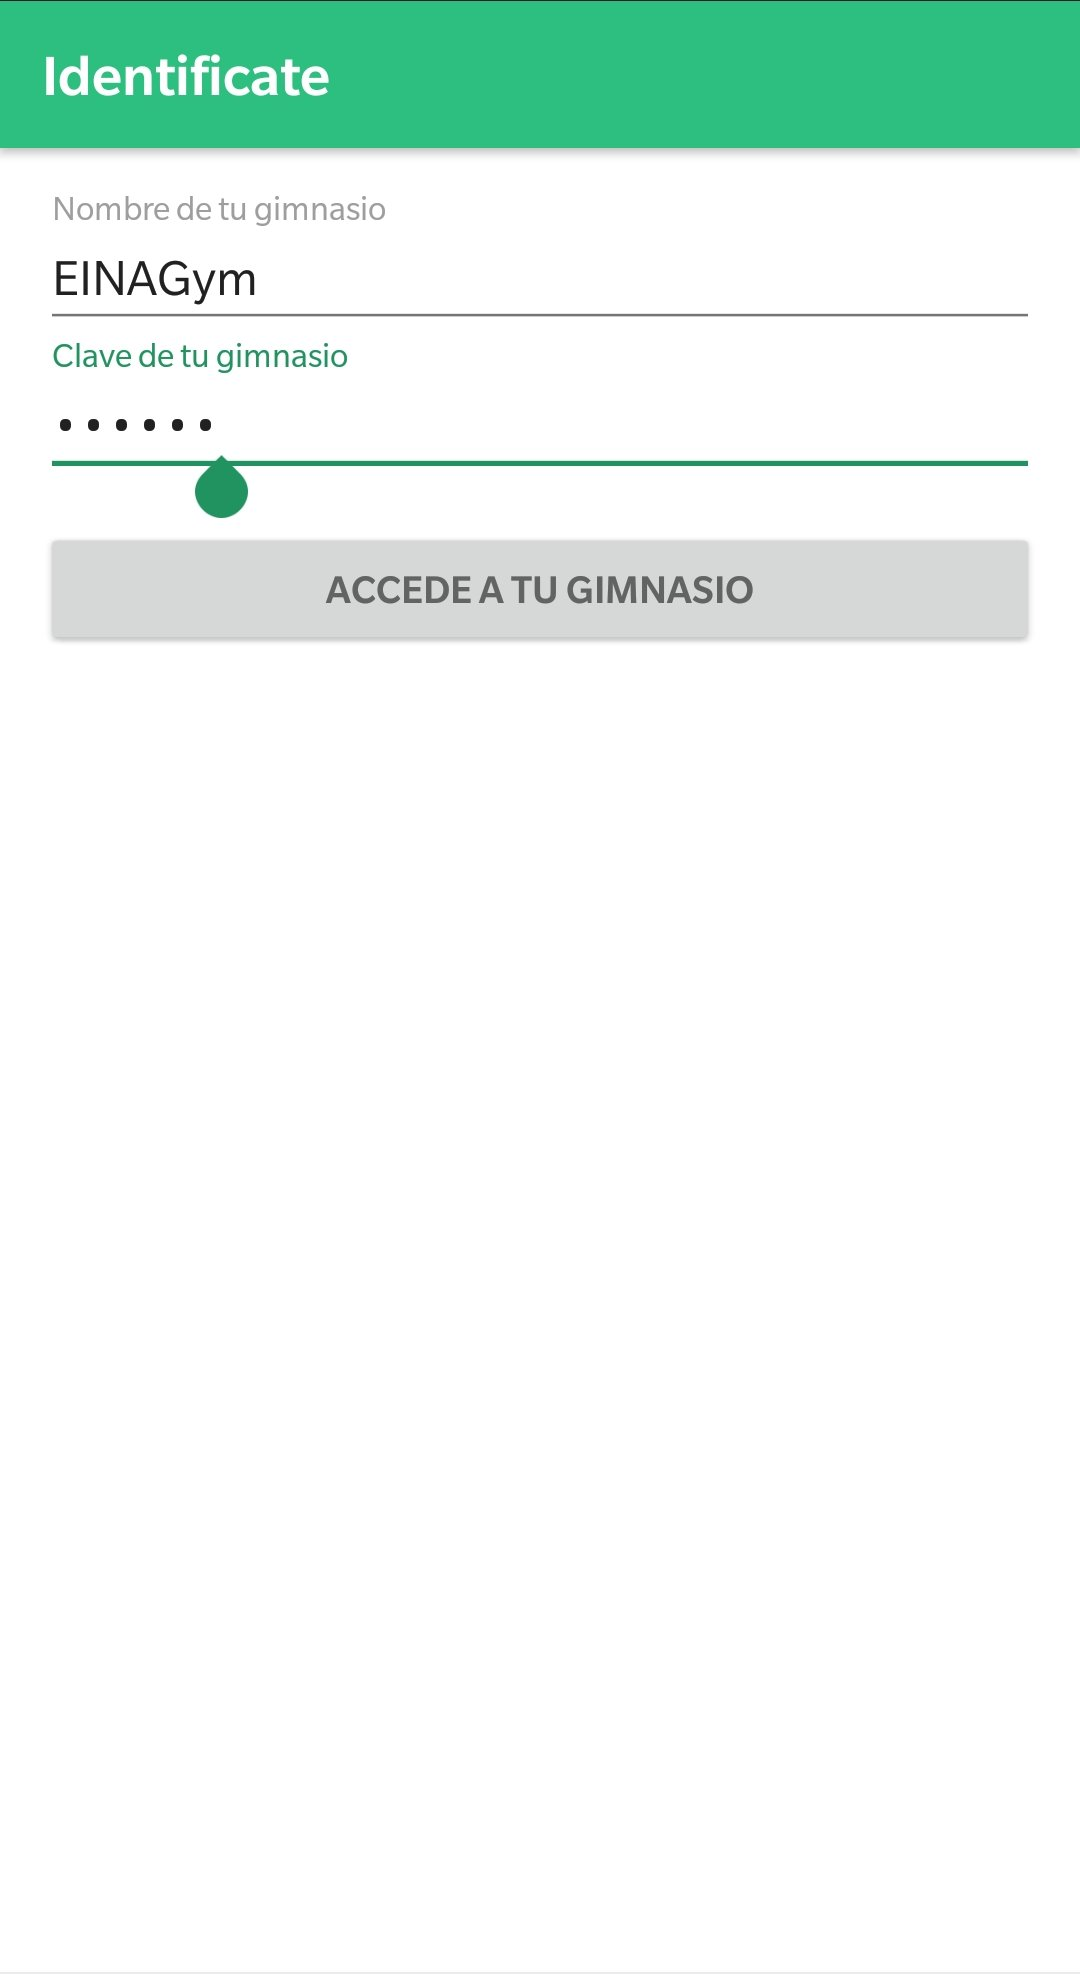
\includegraphics[width=0.3\textwidth]{graficos/manual/IdentificacionPremium.jpg}
	\caption{Acceso premium}
\end{figure}
Una vez accedido al sistema premium, se le presentará a los usuarios una lista de rutinas del gimnasio

\subsubsection{Servicio premium}
\begin{figure}[H]
	\centering
	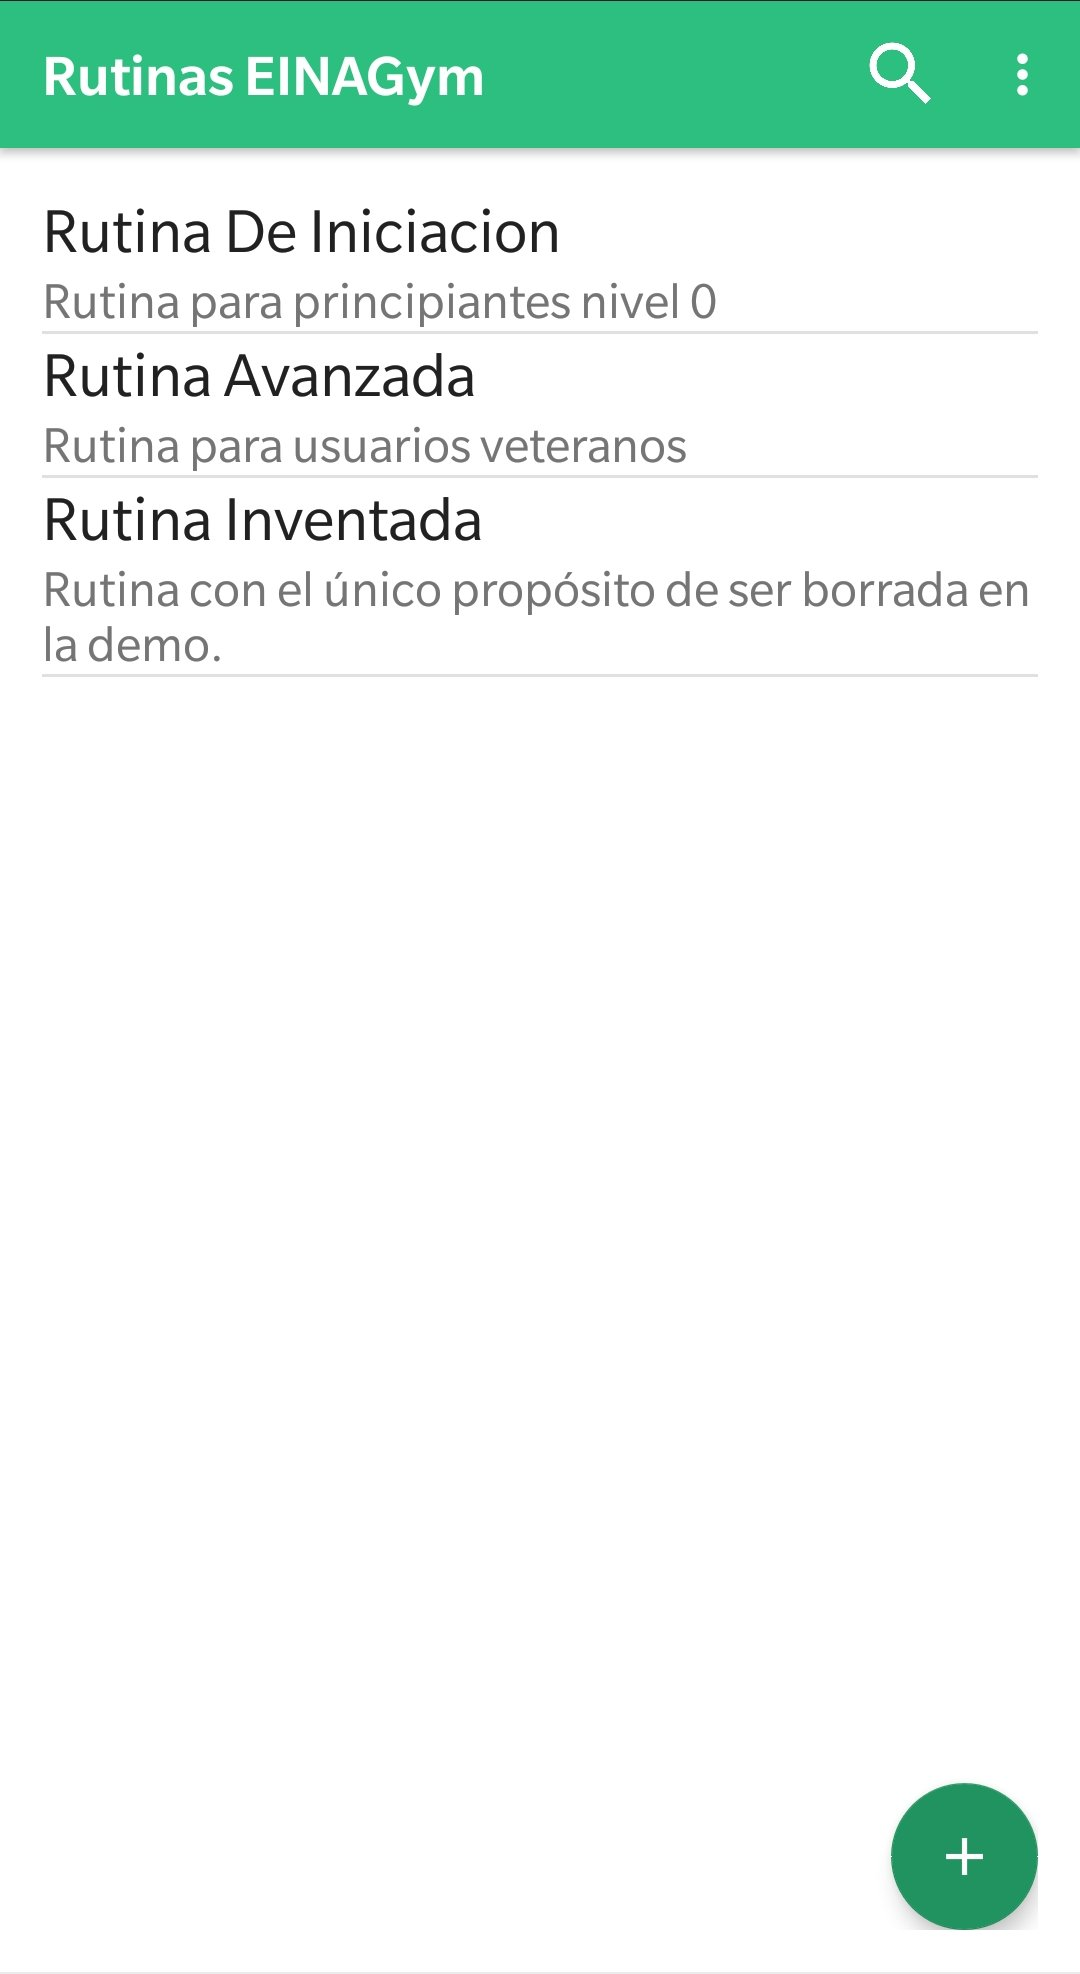
\includegraphics[width=0.3\textwidth]{graficos/manual/RutinasPremium.jpg}
	\caption{Lista de rutinas premium}
\end{figure}
La interfaz es igual a la parte free, pero la única diferencia es que en la barra de acción de Android, se incluye el nombre del gimnasio al cual el usuario pertenece.
A nivel de funcionalidad, la interfaz funciona igual que en la parte gratuita, pero los dos usuarios tienen distintos permisos para modificar las rutinas:
\begin{enumerate}
	\item Los usuarios del gimnasio, sólo pueden ver, filtrar y ejecutar rutinas.
	\item Los entrenadores del gimnasio, pueden realizar todas las acciones de un usuario normal, más la creación, modificación y eliminación de las rutinas.
\end{enumerate}
\begin{figure}[H]
	\centering
	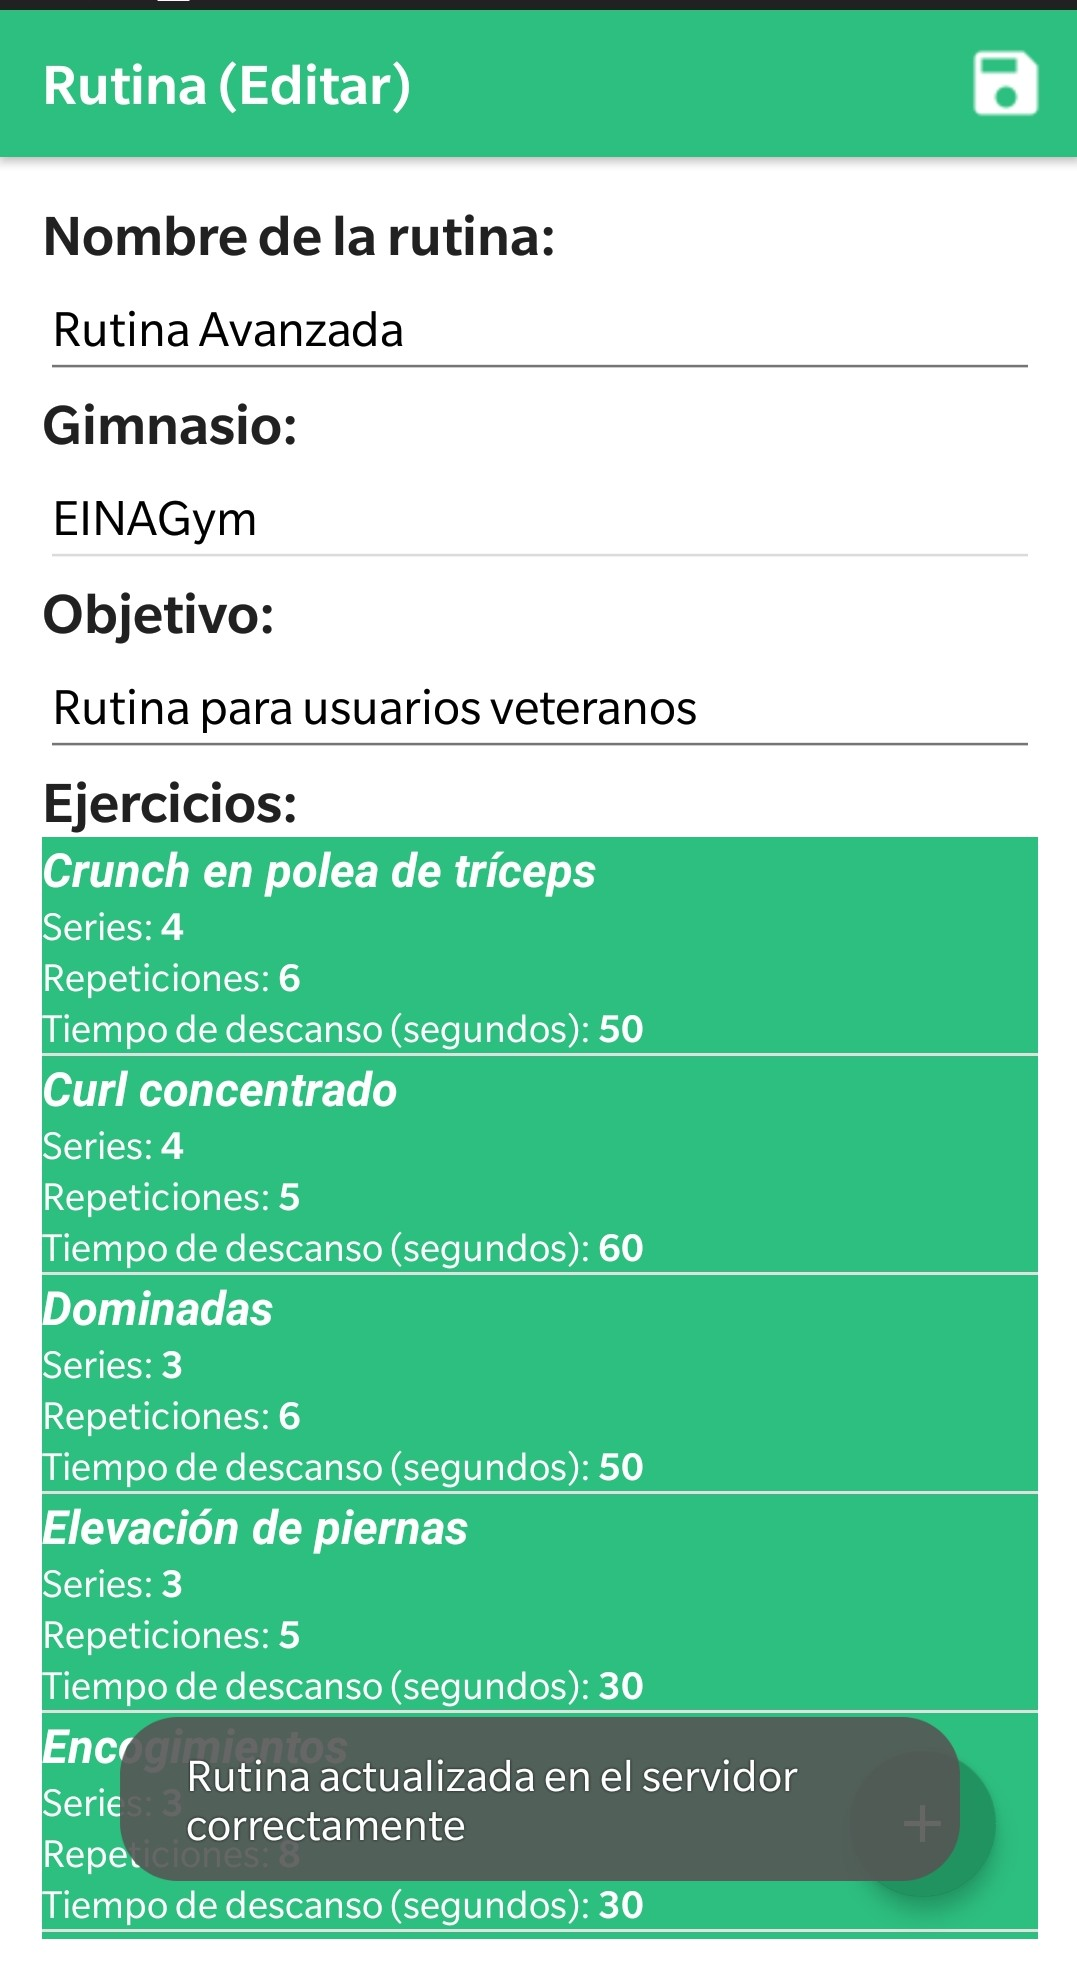
\includegraphics[width=0.3\textwidth]{graficos/manual/EditarRutinaPremium.jpg}
	\caption{Editar Rutina Premium}
\end{figure}
Además, la aplicación informará de todos los cambios realizdos a los entrenadores personales, mediante un diálogo en el que le indicará si las operaciones se han podido realizar en el servidor o ha habido algún problema de red.

\end{document}    